\documentclass{article}

\usepackage{neurips_2026}

\usepackage[utf8]{inputenc}
\usepackage[T1]{fontenc}
\usepackage{hyperref}
\usepackage{url}
\usepackage{booktabs}
\usepackage{amsfonts}
\usepackage{amsmath}
\usepackage{nicefrac}
\usepackage{microtype}
\usepackage{xcolor}
\usepackage{graphicx}
\usepackage{subcaption}
\usepackage{multirow}

\title{PlasmidLM: A Promptable DNA Language Model\\via Verifiable-Reward Post-Training}

\author{%
  Anonymous Author(s)
}

\begin{document}

\maketitle

\begin{abstract}
  Generative DNA models are typically next-token completers: they extend a sequence
  but offer no native interface for telling the model what to make. PlasmidLM is a
  promptable DNA language model for plasmids. A designer supplies a human-readable
  component specification, for example a high-copy \textit{E.~coli} vector with
  kanamycin resistance and an EGFP reporter, and the model generates the corresponding
  multi-kilobase construct in a single autoregressive pass. Prompts are unordered sets
  of named-part tokens at the granularity of biological shorthand, not learned latent
  codes or rigid grammars. We measure outputs along two axes: a sequence is
  \emph{viable} if structurally plausible as a plasmid, and \emph{faithful} if its
  detected components match the prompt; we summarise their conjunction as the
  \emph{useful-plasmid rate}. On a held-out $1{,}000$-prompt benchmark, the post-trained
  model produces useful plasmids in $48.5\%$ of single-shot generations, and in $89.7\%$
  of best-of-$4$ generations under rejection sampling against the same automated
  annotation pipeline used for evaluation. Verifiable-reward post-training with GRPO
  against a $660$-entry sequence motif registry improves on the supervised promptable
  base across all sampling budgets.
  We release the $19.3$M-parameter model, evaluation suite, and a paired benchmark of
  $8{,}000$ prompt-sequence pairs.
\end{abstract}

%% ============================================================
\section{Introduction}
\label{sec:intro}

Designable DNA is the task of taking a high-level specification of a desired construct
and producing a sequence that realises it. It is the daily work of synthetic biology,
from cloning and antigen design to gene-therapy vector assembly and CRISPR guide-vector
pipelines. Genomic language models do not natively support
it. Nucleotide Transformer~\citep{dalla2023nucleotide},
DNABERT-2~\citep{zhou2024dnabert2}, and HyenaDNA~\citep{nguyen2024hyenadna} are
pretrained for discriminative downstream tasks (variant-effect prediction, regulatory
annotation) and expose no generative interface. Evo~2~\citep{brixi2025evo2} is the most
ambitious recent generative effort: it operates at genome scale and accepts a small
catalogue of species tags as prefix conditioning, but is otherwise a sequence completer.
A handful of conditional generators target short regulatory
elements~\citep{sample2019promoter,stark2024dirichlet,taskiran2024cre}, but at the level
of an entire multi-kilobase construct we are not aware of any prior DNA model that
accepts a human-readable component specification and returns a candidate sequence
intended to satisfy it.

Promptable generation calls for a different evaluation than completion. Perplexity
scores how well a model continues a sequence; it does not score whether the sequence
satisfies a specification. We separate two axes. A sequence is \emph{viable} if it is
structurally plausible as a plasmid: a full complement of essential elements arranged in
a configuration compatible with replication and expression. A sequence is
\emph{faithful} if its detected components match the components requested in the prompt.
Their conjunction is the \emph{useful-plasmid rate}, the primary metric we report.
Faithfulness is currently absent from the genomic-LM literature because there are no
standard DNA models with prompts to be faithful to.

Plasmids are a deliberate testbed for this question. They are compact (typically
4 to 10 kb), modular, deposited at scale with lab-supplied metadata, and amenable to
fully automated annotation: an existing pipeline (pLannotate~\citep{mcguffie2021plannotate})
can identify origins, selection markers, regulatory elements, and reporters in a
candidate sequence and return a structured component list. The Addgene repository
contributes over $100{,}000$ sequenced plasmids deposited by working laboratories, each
carrying lab-supplied metadata about its intended use. Crucially, the same pipeline that
scores faithfulness at evaluation time supplies the verifiable reward used during
post-training, so the model is reinforced for the property that is being measured.

This paper makes three contributions. \emph{Promptable DNA generation:} PlasmidLM is a
$19.3$M-parameter plasmid language model that accepts a human-readable component
specification as a prompt and generates a candidate multi-kilobase construct in a single
autoregressive pass. \emph{An evaluation framework for promptable DNA:} the
viable/faithful decomposition and the useful-plasmid rate as a summary metric, grounded
in a $660$-entry motif registry that ties human-readable token names to concrete
sequence-level references. \emph{Verifiable-reward post-training for DNA:} GRPO against
the same registry used for evaluation, which improves the useful-plasmid rate across
single-shot and best-of-$K$ decoding. The post-trained model produces useful plasmids
in $48.5\%$ of single-shot generations and in $89.7\%$ of best-of-$4$ generations on a
held-out $1{,}000$-prompt benchmark.

%% ============================================================
\section{Related work}
\label{sec:related}

\subsection{Generative DNA models}
\label{sec:related-dna}

Genomic language modelling spans a wide range of objectives and scales. The
longest-standing thread is discriminative pretraining: Nucleotide
Transformer~\citep{dalla2023nucleotide}, DNABERT-2~\citep{zhou2024dnabert2}, and
HyenaDNA~\citep{nguyen2024hyenadna} use masked or next-token pretraining and are
evaluated primarily on downstream tasks such as variant-effect prediction. They expose
no generative interface. Evo~\citep{evo2024} introduced large-scale autoregressive
pretraining over bacterial genomes, and Evo~2~\citep{brixi2025evo2} extends the recipe
to a $40$B-parameter model trained across all domains of life with a small fixed
catalogue of species tags that can be prepended to the context. From a designer's
perspective Evo~2 is still a sequence completer: a specification like ``a high-copy
\textit{E.~coli} vector with kanamycin resistance and an EGFP reporter'' has no
representation in its prompt vocabulary. Conditional generators that do offer some prompt
interface have historically been restricted to short regulatory elements: $5'$-UTR
design from massively parallel expression assays~\citep{sample2019promoter}, ribosome
binding-site optimisation~\citep{salis2009}, discrete-diffusion enhancer and promoter
generation~\citep{stark2024dirichlet}, and cell-type-conditional enhancer
design~\citep{chen2024leonine,taskiran2024cre}. These methods operate on isolated
elements of $\sim\!100$ to $1{,}000$ bp and target either a single scalar objective
(e.g.\ expression level, TF binding score) or a single contextual condition (e.g.\ cell
type). The coordination constraints that arise when an entire multi-kilobase construct
must simultaneously contain a compatible origin, selection marker, regulatory cassette,
and payload are not addressed at this scale. In the protein domain, conditional
generation is further along, with family-conditional models~\citep{madani2023progen}
and discrete-diffusion approaches~\citep{alamdari2023evodiff} demonstrating controllable
single-chain generation; the analogous problem for DNA at the construct level has
remained open.

\subsection{Instruction tuning and RL for sequence design}
\label{sec:related-rl}

Outside biology, the recipe of post-training a pretrained autoregressive model to follow
user specifications is now standard. Supervised instruction tuning on prompt-response
pairs~\citep{wei2022flan} produces models that generalise to unseen tasks, and
reinforcement learning from human or automated
feedback~\citep{christiano2017preferences,stiennon2020summarization,ouyang2022instructgpt}
further aligns model behaviour with a desired specification. PPO-based RLHF, direct
preference optimisation~\citep{rafailov2023dpo}, and group-relative policy optimisation
(GRPO)~\citep{shao2024deepseekmath} are the dominant algorithmic variants; the latter
has driven substantial gains on tasks where outcomes can be \emph{verified}
automatically, most prominently mathematical
reasoning~\citep{shao2024deepseekmath,lightman2024prm} and open-ended post-training
recipes~\citep{lambert2024tulu}. The same paradigm has begun to migrate into biological
sequence design: GFlowNets for protein generation~\citep{jain2022gflownet},
RL for small-molecule drug design~\citep{zhou2023molrl}, GRPO for RNA inverse
folding~\citep{yangheng2024rnagrpo}, and RL-driven optimisation of cis-regulatory
elements~\citep{taskiran2024cre}. The reward signals there span scalar property models,
folding-energy and structure-prediction surrogates, and oracle assays; the unifying
feature is differentiable or verifiable scoring on a single short sequence. Our
contribution sits in parallel to text language modelling rather than to those
sequence-design lines: we apply the same supervised-then-reinforced post-training
pattern that turns a text LM into an instruction follower to a DNA LM, where the
specification is a list of named components, the reward is a sequence-annotation
pipeline, and the unit of generation is a multi-kilobase construct rather than a short
element.

%% ============================================================
\section{Methods}
\label{sec:methods}

\subsection{Dataset construction}
\label{sec:data}

Plasmid sequences were drawn from the Addgene repository, yielding a corpus of 108,448
unique plasmids after deduplication and length filtering. Each sequence was annotated
using pLannotate~\citep{mcguffie2021plannotate}, which queries four curated databases via
BLAST and DIAMOND: the GenoLIB/SnapGene feature database, FPbase (fluorescent proteins),
Swiss-Prot (general proteins), and Rfam (non-coding RNAs).

\subsection{Special token design}
\label{sec:tokens}

The token vocabulary is the prompt interface, and it is the design choice that turns a
sequence completer into a promptable model. Lab scientists describe plasmids at two
granularities: specific named parts where exact identity matters operationally
(ampicillin resistance and chloramphenicol resistance are not interchangeable in a
clone), and directional categories where designers think in classes rather than parts
(high versus low copy, mammalian versus bacterial vector). Any prompt vocabulary that
does not match both granularities forces the designer to translate intent into a
foreign idiom. We built the vocabulary backwards from designer practice: assembling
annotations from pLannotate~\citep{mcguffie2021plannotate}, metadata from
Addgene~\citep{addgene2024}, and any other available signal, then asking at each
granularity what a designer would want to specify. The hard/soft split is the empirical
consequence of this exercise rather than an a priori architectural choice. Hard tokens
are sequence-checkable and can ground a verifiable reward; soft tokens encode
metadata-level context that no alignment can confirm. GRPO with sequence-level rewards
is impossible without this distinction, and the boundary along which designers' mental
model factors happens to coincide with the boundary along which the available reward
signal factors. A motif registry ($660$ entries) bridges human-readable token names to
the gene-level identifiers used by pLannotate.

The token vocabulary is divided into two classes with distinct roles. \emph{Hard tokens}
(57 types, seven categories) represent sequence-verifiable genetic components and are the
target of both the GRPO reward and evaluation: origins of replication (\texttt{ORI\_}),
antibiotic resistance markers (\texttt{AMR\_}), promoters (\texttt{PROM\_}), general
regulatory and structural elements (\texttt{ELEM\_}), reporters (\texttt{REPORTER\_}),
replication proteins (\texttt{REP\_}), and epitope tags (\texttt{TAG\_}). Token names use
human-readable identifiers at the specificity level of a named part rather than gene
family (e.g., \texttt{<ORI\_COLE1>}, \texttt{<AMR\_AMPICILLIN>}, \texttt{<REPORTER\_GFP>}).

\emph{Soft tokens} represent metadata-level context that cannot be verified by sequence
alignment alone and are therefore excluded from the GRPO reward and fidelity evaluation,
but present in training prompts to provide additional conditioning signal. They include
vector type (\texttt{VEC\_}: e.g., \texttt{<VEC\_MAMMALIAN>},
\texttt{<VEC\_LENTIVIRAL>}), host species (\texttt{SP\_}: \texttt{<SP\_HUMAN>},
\texttt{<SP\_ECOLI>}, etc.), copy number (\texttt{<COPY\_HIGH>}, \texttt{<COPY\_LOW>}),
and backbone identity (\texttt{BB\_}). These are derived from Addgene metadata fields
rather than sequence annotation.

A key design decision is the \emph{motif registry}: a curated lookup table mapping each
hard token to the specific pLannotate sequence-level entries (sseqids) that correspond to
it. This bridge is necessary because token names use biological shorthand (e.g.,
\texttt{AMR\_AMPICILLIN}) while pLannotate uses gene-level identifiers (e.g.,
\texttt{AmpR}, \texttt{AmpR\_(2)}). Many named components have multiple sequence variants
in the annotation database (codon-optimized forms, truncated constructs carried along
from earlier cloning histories, and sequences from different source organisms), so the
registry maps each of the 57 token types to all qualifying variants. After filtering,
the registry contains 660 sequence-level entries in total, with each of the 57 surviving
token types attested in at least 309 training plasmids. The same registry is used both to define the GRPO
training reward and to compute the evaluation fidelity metric, ensuring evaluation
directly measures what was reinforced during training. Each training example takes the form:
\[
  \texttt{<BOS>}\ \underbrace{\langle \mathrm{tok}_1 \rangle \cdots \langle
  \mathrm{tok}_k \rangle}_{\text{component
  prompt}}\ \texttt{<SEQ>}\ \underbrace{\mathrm{ATGGCC}\ldots}_{\text{6-mer tokenized
  DNA}}\ \texttt{<EOS>}
\]
where the component tokens are sorted canonically and the \texttt{<SEQ>} token marks the
transition from prompt to sequence. This format conditions generation at inference time
by supplying the desired token list; the model generates the DNA completion autoregressively.

\begin{figure}[t]
  \centering
  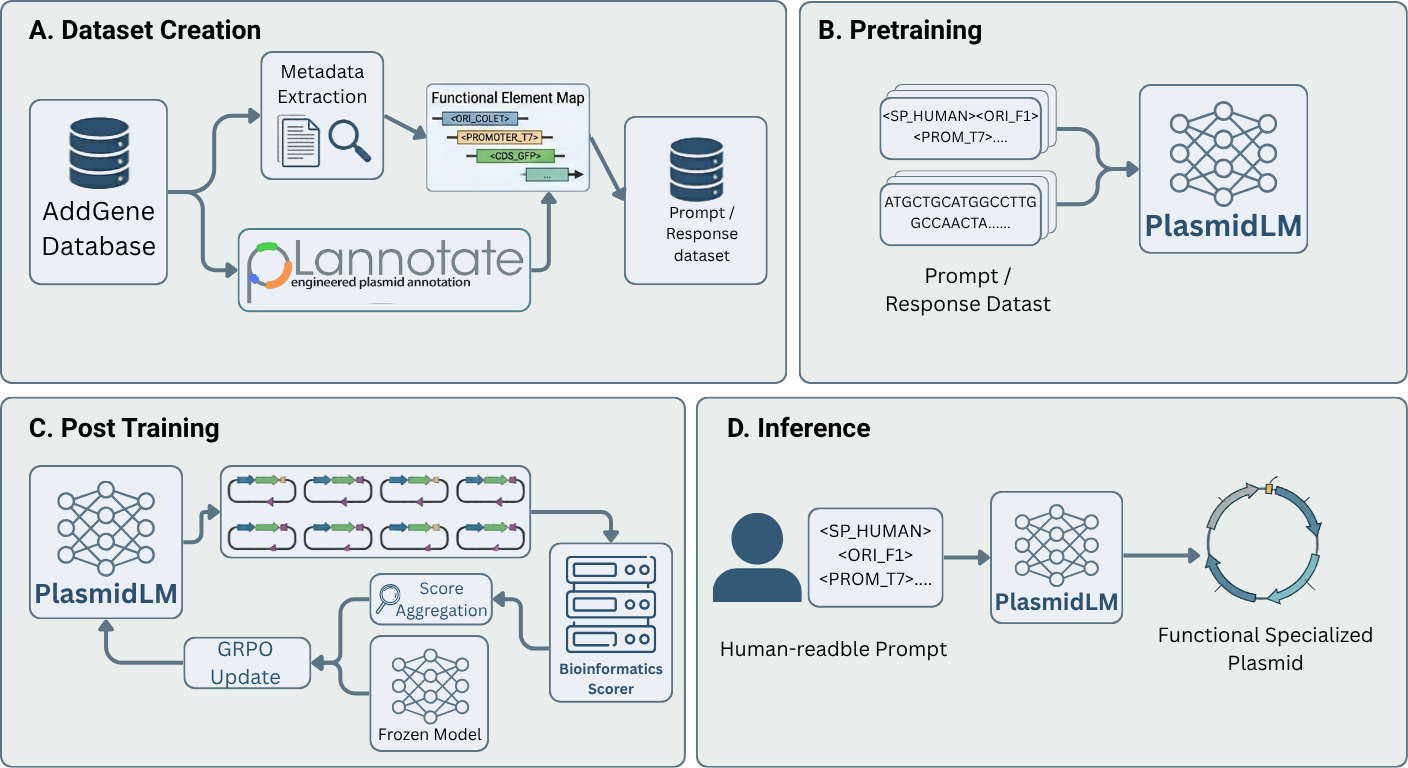
\includegraphics[width=0.95\linewidth]{figures/plasmidlm_process.png}
  \caption{PlasmidLM training and inference pipeline. \textbf{(A)} Raw Addgene plasmid
    sequences are annotated with pLannotate to identify functional elements, which are
    mapped to hard component tokens (e.g., \texttt{<ORI\_COLE1>}) via the motif registry
    and supplemented with soft metadata tokens (vector type, species, copy number).
    \textbf{(B)} Prompt-paired training: the full sequence is paired with its token prompt
    and trained with next-token prediction. \textbf{(C)} GRPO post-training: the policy
    generates $G=8$ completions per prompt, scored by BLAST alignment against the motif
    registry; group-normalized rewards update the policy with a KL constraint to the frozen
    reference. \textbf{(D)} Inference: a user-supplied token list conditions generation
  autoregressively.}
  \label{fig:pipeline}
\end{figure}

\subsection{Model architecture and pretraining}
\label{sec:pretraining}

PlasmidLM is a decoder-only transformer with 19.3 million parameters: hidden dimension
$384$, $10$ layers, $8$ attention heads of head dimension $48$, rotary positional
embeddings (RoPE), RMSNorm, and weight tying between the input embedding and the
language modeling head. A custom 6-mer tokenizer produces a vocabulary of $4{,}096$ DNA
k-mers plus special tokens, and a maximum positional context of $16{,}384$ tokens
supports the multi-kilobase plasmids in our corpus. Pretraining used standard
next-token prediction on the full Addgene corpus to step $15{,}000$ (batch size $64$,
AdamW, cosine schedule peaking at $3\times10^{-4}$), with the released checkpoint
reaching eval loss $0.101$ and token accuracy $95.8\%$.

\subsection{GRPO post-training}
\label{sec:grpo}

To sharpen prompt fidelity beyond what supervised pairing achieves, we apply Group
Relative Policy Optimization (GRPO)~\citep{shao2024deepseekmath}. For each training
prompt, the policy generates $G=8$ candidate completions. Each completion is scored by a
composite reward: for every requested component token, BLAST is run against the
corresponding motif registry reference sequences, and partial credit is awarded based on
percent identity, alignment coverage, and normalized bit score. An aggregate recall
penalty ensures sequences that miss components entirely receive low reward regardless of
per-hit quality. Rewards are group-normalized to compute advantages, and a clamped KL
penalty ($\beta=0.5$) applied to the frozen reference policy stabilizes training. Full
hyperparameters are in Appendix~\ref{app:model}.

%% ============================================================
\section{Evaluation framework}
\label{sec:eval}

\subsection{Two evaluation axes}
\label{sec:eval-axes}

A promptable model needs an evaluation that scores both whether the output is a
plausible thing of the right kind and whether it satisfies the prompt. We separate the
two and report their conjunction.

\textbf{Viable.} A generated sequence is \emph{viable} iff
pLannotate~\citep{mcguffie2021plannotate} detects an origin of replication, a selection
marker, and at least one of a promoter or a coding sequence. Terminators and CDSs are
recorded for descriptive purposes but do not gate viability. Let $V_i \in \{0,1\}$
denote the viability indicator for prompt $i$'s generated sequence.

\textbf{Faithful.} For each hard token $t$ requested in prompt $i$, the token is
\emph{recovered} iff the set of pLannotate sseqids attributed to $t$ by the motif
registry intersects the set of sseqids that pLannotate detects in the candidate
sequence. The $\geq\!95\%$ identity and $\geq\!80\%$ coverage thresholds appear at
\emph{registry construction} time (Section~\ref{sec:tokens}), where they decide which
reference variants qualify as canonical exemplars of $t$; per-prompt scoring is then a
set-intersection on already-qualified sseqids, which is the same rule used by the GRPO
reward. Per-prompt faithfulness is $F_i = n_{\text{found},i} / n_{\text{requested},i}$,
defined for prompts with $n_{\text{requested},i} > 0$ ($996$ of $1{,}000$).

\textbf{Useful-plasmid rate.} The conjunction of the two axes is the headline summary
metric. A sequence is \emph{useful at threshold $T$} iff it is viable \emph{and}
achieves $F_i \geq T$: $U_i^{(T)} = V_i \wedge \mathbf{1}[F_i \geq T]$. Viability alone
(equivalently $T{=}0$) cannot distinguish a sequence that ignores the prompt from one
that follows it; faithfulness alone rewards sequences that concatenate the requested
motifs on an unstable backbone. Throughout we use $T{=}0.5$ as the default summary
threshold because at-least-half of requested components present is a reasonable
user-facing minimum for a prompt-following system; the threshold sweep in
Appendix~\ref{app:results} reports the full range and the GRPO advantage at every
positive $T$.

\subsection{Annotation pipeline and motif registry}

Sequences are annotated with pLannotate (named-feature detection via BLAST/DIAMOND
against four curated databases~\citep{mcguffie2021plannotate}), Prodigal (ORF prediction
in metagenomic mode), and dustmasker (low-complexity intervals). The motif registry
operates at two levels: $660$ sequence-level entries (individual reference variants)
grouped into $57$ component types (named parts such as \texttt{ORI\_COLE1} or
\texttt{AMR\_AMPICILLIN}); see Section~\ref{sec:tokens}. Running this exact pipeline on
real training plasmids recovers $71.8\%$ of requested tokens (token-pooled across
prompts), establishing a practical detection ceiling that bounds any model's
faithfulness score from above. The remaining $28.2\%$ are tokens whose references are
too short to clear BLAST's bit-score threshold (most epitope tags), or whose
codon-optimised variants fall below the identity threshold. The viability rate on the
same real-plasmid panel is $95.0\%$ under our viability rule. Faithfulness numbers in
this paper are therefore most usefully read against these two same-pipeline ceilings
rather than against an idealised $100\%$.

\subsection{Sampling protocols}
\label{sec:sampling}

We evaluate generations under two sampling regimes. The \emph{single-shot} regime draws
one sample per prompt at temperature $0.7$, top-$p{=}0.95$, top-$k{=}50$, and is the
default for headline numbers. The \emph{best-of-$K$} regime draws $K$ independent
samples per prompt and keeps the candidate with the highest annotation-pipeline
$n_{\text{found}}$ score, breaking ties by viability then faithfulness. This is realistic
for users with access to the same annotation pipeline at inference time, who can run
pLannotate on candidates and reject failures; we report $K\in\{1, 2, 4\}$ with four
independent seeds per $K$. Where we contrast the post-trained model with the supervised
promptable base, both checkpoints generate one sample per prompt on the same $1{,}000$
held-out prompts under identical sampling hyperparameters, supporting paired statistical
tests on prompt-level outcomes.

\paragraph{Statistical conventions.}
Confidence intervals, paired-test conventions, and per-category caveats are documented
in Appendix~\ref{app:stats}.

\subsection{What the model emits}
\label{sec:exemplars}

A reader unfamiliar with plasmid annotation may benefit from seeing what the model
actually emits before turning to aggregate metrics. Figure~\ref{fig:exemplars} shows
three exemplar generations spanning the quality range: a clean success ($f_i = 1.00$,
all five requested hard tokens recovered, plasmid structurally coherent as a
mammalian/\textit{E.~coli} shuttle), a typical single-shot result ($f_i = 0.50$, three
of six tokens recovered, structurally plausible plasmid on a different backbone than
requested), and a failure case ($f_i = 0.40$, model received \texttt{COPY\_LOW} +
\texttt{ORI\_P15A} + \texttt{AMR\_CHLORAMPHENICOL} but emitted a high-copy ColE1 origin
and ampicillin resistance). The failure case concretises the soft-token and
rare-hard-token failure modes analysed in Sections~\ref{sec:prompt-fid}
and~\ref{sec:soft-tokens}. The three rows are not selected to flatter the model; they
are intended to span the empirical quality distribution that the aggregate numbers
summarise.

\begin{figure}[t]
  \centering
  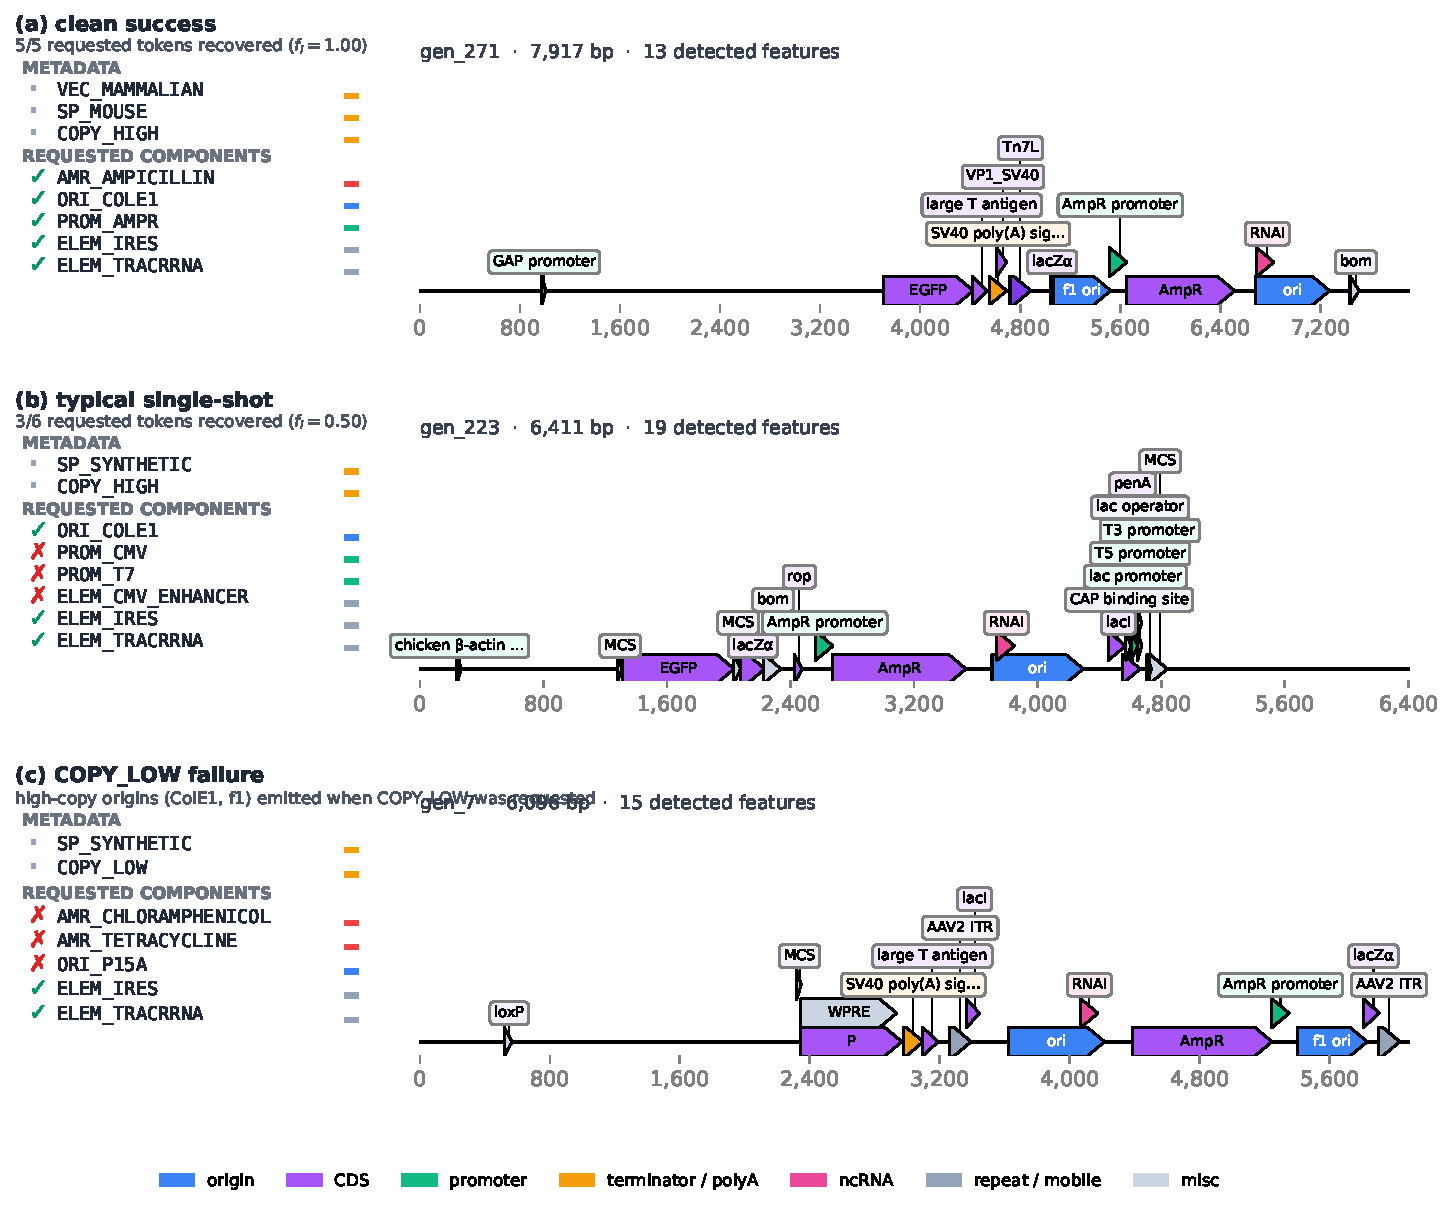
\includegraphics[width=\linewidth]{figures/exemplar_gallery.pdf}
  \caption{Three exemplar generations spanning the quality range. Each row: prompt
    component list (left) and pLannotate annotation map (right), coloured by feature
    type. (a) \texttt{gen\_271}, clean success: $5/5$ hard tokens recovered, plasmid
    is a coherent mammalian/\textit{E.~coli} shuttle vector. (b) \texttt{gen\_223},
    typical single-shot: $3/6$ tokens recovered, structurally plausible plasmid on a
    different backbone than requested. (c) \texttt{gen\_7}, \texttt{COPY\_LOW} +
    rare-AMR failure: prompt asked for low-copy + chloramphenicol/tetracycline
    resistance; model emitted high-copy origins and ampicillin resistance instead.}
  \label{fig:exemplars}
\end{figure}

\subsection{Headline result: the useful-plasmid rate}
\label{sec:useful}

\begin{table}[t]
  \caption{Useful-plasmid rate ($T{=}0.5$) on the held-out $1{,}000$-prompt benchmark.
    Single-shot uses temperature $0.7$, top-$p{=}0.95$, top-$k{=}50$; best-of-$K$ ranks
    $K$ independent draws per prompt by the annotation pipeline (oracle ranker, four
    seeds). The real Addgene reference panel admits no useful rate at $T{=}0.5$ because
    real plasmids have no original prompt to be faithful to; the same pipeline reports
    structural plausibility of $95.0\%$ on the panel and $0.0\%$ on random and
    dinucleotide-shuffled controls (compare Figure~\ref{fig:bok}, left panel).}
  \label{tab:useful_main}
  \centering
  \small
  \begin{tabular}{lccc}
    \toprule
    & Single-shot & Best-of-$2$ & Best-of-$4$ \\
    \midrule
    PlasmidLM (post-GRPO) & $\mathbf{48.5\%}$ & $\mathbf{73.6\%}$ & $\mathbf{89.7\%}$ \\
    PlasmidLM (supervised base) & $38.7\%$ & $60.4\%$ & $78.9\%$ \\
    Random GC-matched / shuffled & $0.0\%$ & --- & --- \\
    \bottomrule
  \end{tabular}
\end{table}

\begin{figure}[t]
  \centering
  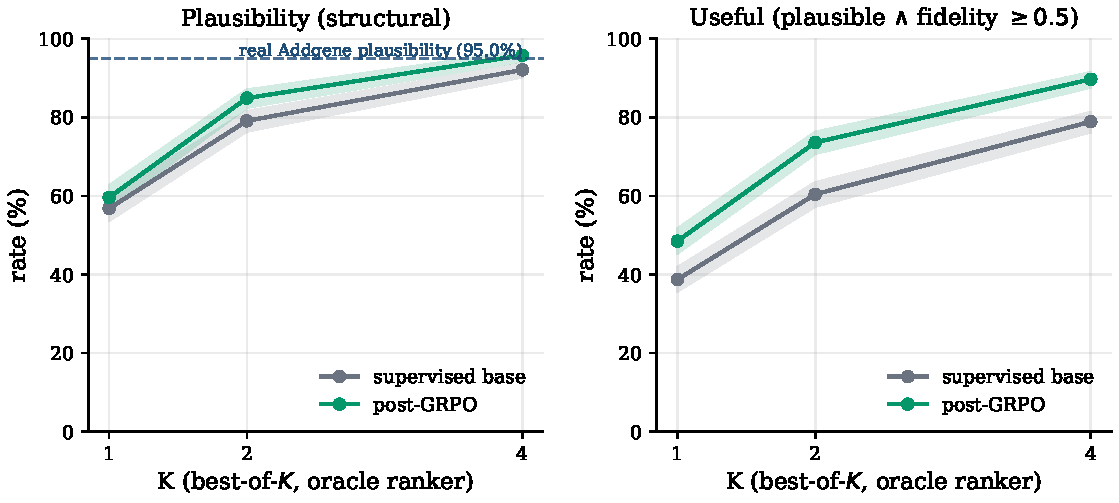
\includegraphics[width=\linewidth]{figures/bok_useful_curve.pdf}
  \caption{Best-of-$K$ for $K \in \{1, 2, 4\}$ on the paired $n{=}1{,}000$ benchmark,
    oracle ranker. Left: structural plausibility, with the dashed line marking the
    real-Addgene plausibility rate ($95.0\%$). Right: useful-plasmid rate ($T{=}0.5$).
    Wilson $95\%$ bands shaded. Post-GRPO is strictly above the supervised base at every
    $K$ on both metrics; the post-GRPO plausibility curve passes the real-Addgene
    reference at $K{=}4$ ($95.8\%$). The useful-rate gap stays in the $+9.8$ to
    $+13.2$~pp range across $K$. The reference line is plausibility only --- useful-rate
    at $T{=}0.5$ is not defined for real Addgene because real plasmids have no original
    prompt to be faithful to.}
  \label{fig:bok}
\end{figure}

PlasmidLM produces useful plasmids in $48.5\%$ of single-shot generations and in
$89.7\%$ of best-of-$4$ generations on the held-out $1{,}000$-prompt benchmark
(Table~\ref{tab:useful_main}, Figure~\ref{fig:bok}). Random and dinucleotide-shuffled
controls score $0.0\%$. The same annotation pipeline finds that $95.0\%$ of held-out
real Addgene plasmids are structurally plausible; the post-GRPO plausibility curve
passes that reference at best-of-$4$ ($95.8\%$, Figure~\ref{fig:bok} left), so on the
viability axis post-training closes the gap to natural plasmids when the user can
afford four samples per prompt.

The supervised promptable base, before any verifiable-reward post-training, is already a
useful model: it produces useful plasmids $38.7\%$ of the time at single-shot decoding
and $78.9\%$ at best-of-$4$. Post-training adds $+9.8$ pp at single-shot decoding
(paired bootstrap $95\%$ CI $[+5.7, +13.9]$, McNemar $p \approx 6{\times}10^{-6}$) and
preserves a $+10.8$ pp advantage under best-of-$4$ ($p\approx 2\times 10^{-12}$). The
gain is significant at every positive faithfulness threshold and peaks near $T{=}0.5$
(threshold sweep in Appendix~\ref{app:results}). It is also not explained by sampling
temperature: a sweep of the base model shows faithfulness peaking at $t{=}0.3$ and
degrading at higher temperatures, so the matched $t{=}0.7$ setting is already near the
base's optimum (Appendix~\ref{app:tempsweep}).

%% ============================================================
\section{Analysis}
\label{sec:experiments}

\subsection{Distributional and biophysical structure}
\label{sec:distributions}

The viable/faithful gate metrics treat each plasmid as pass-or-fail. We complement them
with distributional checks against real Addgene at the population level, on properties
the gate metric does not directly examine: length, GC content, codon usage in predicted
ORFs, GC skew variation, ViennaRNA~\citep{lorenz2011viennarna} minimum-free-energy
density, and pairwise $6$-mer diversity (Figure~\ref{fig:distributions}).

\begin{figure}[t]
  \centering
  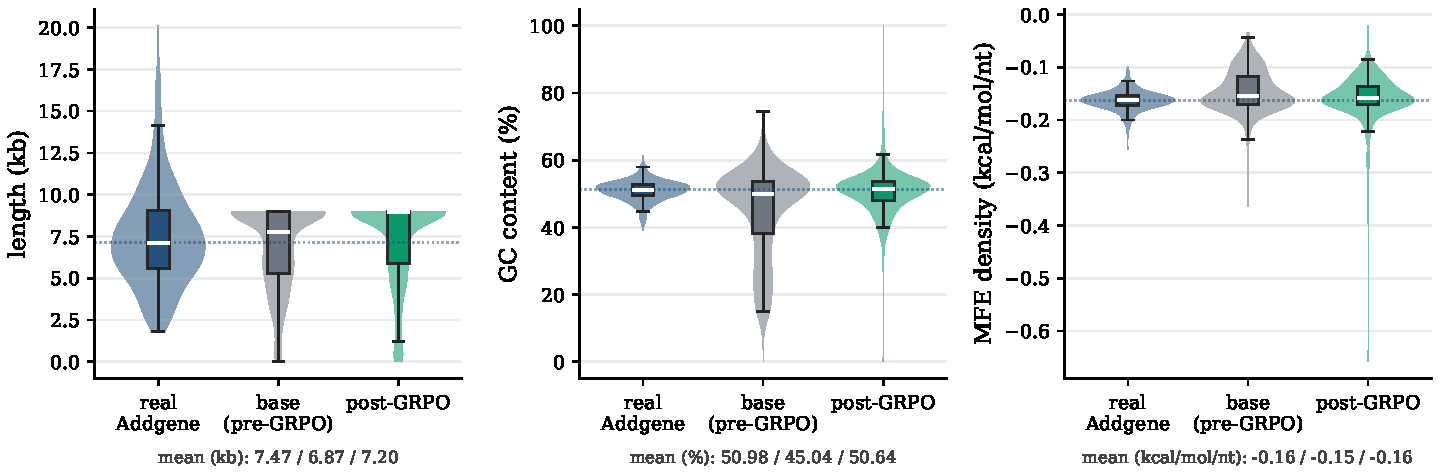
\includegraphics[width=\linewidth]{figures/distribution_violins.pdf}
  \caption{Distributional comparison of generated and real plasmids across length (kb),
    GC content (\%), and ViennaRNA MFE density (kcal/mol/nt). Three populations per
    panel: real held-out Addgene ($n{=}500$), supervised base ($n{=}1{,}000$), and
    post-GRPO ($n{=}1{,}000$). Inner box shows IQR and median; the dotted reference
    line is the real-population median; means are printed under each panel. The GC
    panel shows the headline distributional failure mode: a long low-GC tail in the
    supervised base, driven by a subpopulation of near-all-AT outputs, that
    post-training truncates and replaces with a real-like distribution.}
  \label{fig:distributions}
\end{figure}

Mean lengths are $6.9$~kb (base) and $7.2$~kb (post-GRPO), against an Addgene reference
of $7.5$~kb. The more informative pattern is in GC content: the supervised base
produces a long low-GC tail with mean $45.0\%$ driven by a subpopulation of
near-all-AT outputs, absent from real plasmids; post-training truncates this tail and
recovers a real-like distribution with mean $50.6\%$ (real Addgene mean
$51.0\%$). MFE density~\citep{lorenz2011viennarna} tells the same story: real plasmids
sit at $-0.163$~kcal/mol/nt, the supervised base at $-0.146$, and post-GRPO at
$-0.158$ --- within $3\%$ of the real population (per-sequence ViennaRNA fold under DNA
Mathews~2004 parameters; sequences over $5$~kb are summarised as the mean MFE density
across $5$ random $2$~kb windows; see Appendix~\ref{app:pipeline}). Codon-usage JSD
against \textit{E.~coli} is $0.131$ in predicted open reading frames; GC skew variation
is $0.0566$ versus reference $0.0593$. Generated sequences are at least as diverse as
real plasmids on $6$-mer statistics~\citep{brown2016sourmash}, with zero sourmash
containment hits above threshold $0.3$ in either run, ruling out training-set
memorisation. A LightGBM discriminator separating generated from real plasmids on
sequence-level features achieves AUC $0.937$ to $1.000$ across four post-GRPO seeds and
$1.000$ across all four base seeds; the seed-level variance precludes a strong claim
that post-training reduces separability. Post-training therefore recovers coarse
distributional structure that the supervised base misses; the next subsection looks at
finer-grained codon-level structure conditioned on the prompt.

A separate viability question is whether either checkpoint produces a structurally
plausible plasmid in the first place. Under the rule of Section~\ref{sec:eval-axes}
(origin $\wedge$ selection marker $\wedge$ at least one of promoter or CDS), pass rates
are $59.6\%$ for post-GRPO and $56.8\%$ for the supervised base, against $95.0\%$ for
real Addgene and $0.0\%$ for random and dinucleotide-shuffled controls. The viability
gap between the two checkpoints is not statistically significant (paired bootstrap
$95\%$ CI $[-1.4, +7.1]$~pp, McNemar $p{=}0.21$). Read together with the $+9.8$~pp
useful-plasmid gain ($p \approx 6 \times 10^{-6}$), this gives post-training a clean
interpretation: GRPO does not hurt viability and substantially improves controllability.
The recipe is best understood as a targeted prompt-follower with a known scope, changing
\emph{which} components a viable plasmid contains rather than \emph{whether} the output
is a viable plasmid in the first place.

\subsection{Host-conditional codon usage}
\label{sec:cai}

A registry-independent test of host-species conditioning. For each generated and real
plasmid we predict open reading frames with Prodigal~\citep{hyatt2010prodigal} and
compute the codon adaptation index~\citep{sharp1987cai} of each predicted CDS against
the codon-usage tables of \textit{E.~coli}, \textit{S.~cerevisiae}, human, and mouse
(Kazusa~\citep{nakamura2000kazusa}, whole-CDS frequencies; CAI evaluated over body
codons of ORFs $\geq 100$ codons, then length-weighted within each plasmid). The
\texttt{SP\_*} token in the prompt is a soft token: it is part of the input but never
appears in the GRPO reward, so any host-conditional codon signal must come from
supervised pretraining alone. A model that has learned host-specific codon usage should
produce sequences whose CAI to a given host table tracks the host declared in the
prompt. Sharp--Li CAI is GC-dependent and the four organisms have different GC content,
so we summarise the cleanest contrast as
$\Delta = \mathrm{CAI}_{\mathrm{yeast}} - \mathrm{CAI}_{\mathrm{ecoli}}$ per sequence:
yeast and \textit{E.~coli} have similar GC and different codon preferences, so this
difference isolates the codon-preference signal from the GC confound.

\begin{figure}[t]
  \centering
  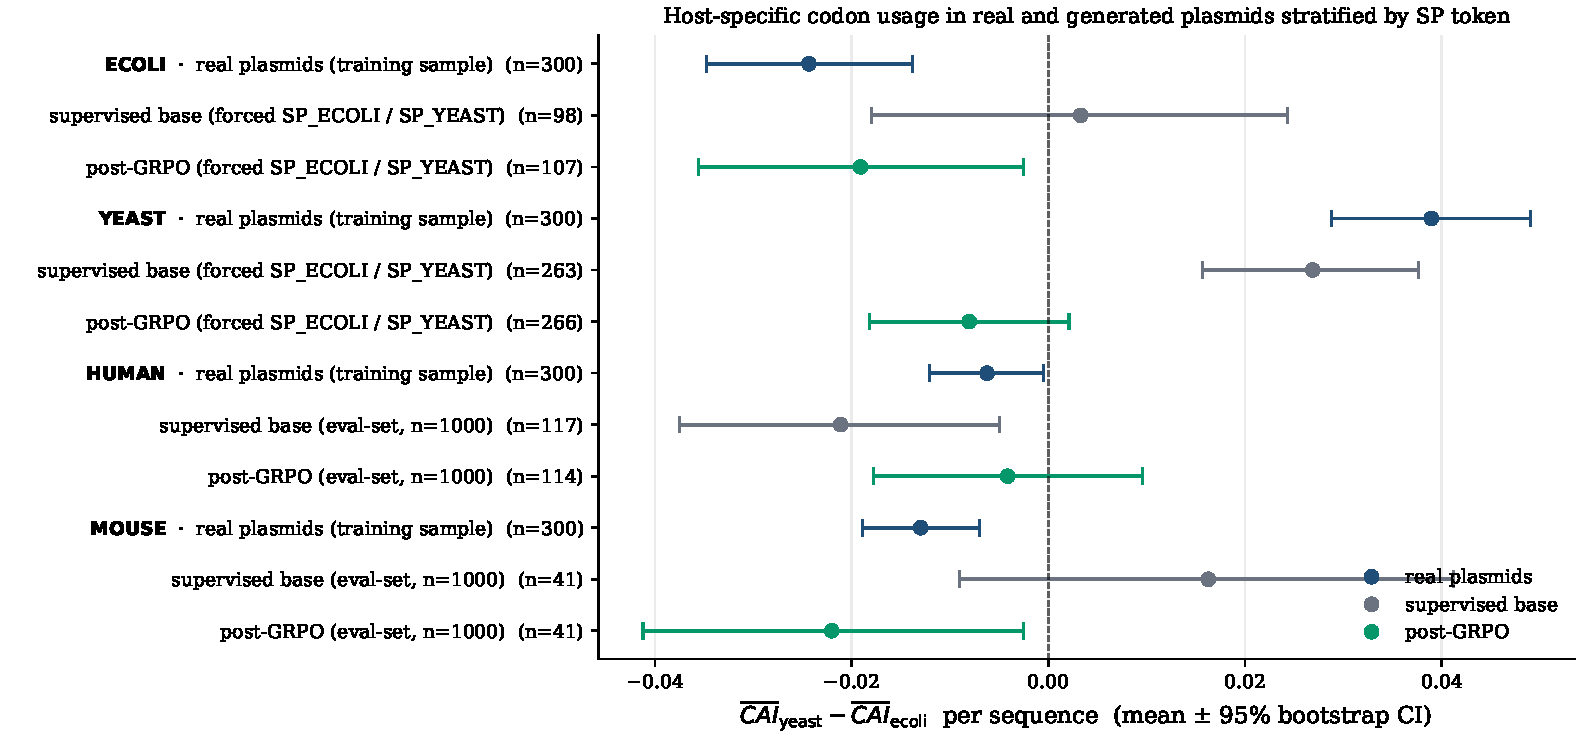
\includegraphics[width=\linewidth]{figures/cai_yeast_minus_ecoli_forest.pdf}
  \caption{Host-conditional codon usage. For each plasmid we compute
    $\Delta = \mathrm{CAI}_{\mathrm{yeast}} - \mathrm{CAI}_{\mathrm{ecoli}}$ across
    predicted ORFs (Prodigal). The yeast-vs-\textit{E.~coli} contrast isolates
    codon-preference signal from the GC confound that affects Sharp--Li CAI. Real
    plasmids show a clean diagonal across four host classes (top section). Generated
    plasmids reproduce the diagonal partially: the post-GRPO model direction-matches
    real plasmids on three of four host classes; the supervised base on two of four.
    Bars are bootstrap $95\%$ CIs over plasmids; rows whose CI excludes zero are
    significant at $p < 0.05$.}
  \label{fig:cai}
\end{figure}

Real plasmids show the expected diagonal across all four hosts ($n{=}300$ training
plasmids per SP class, sampled with their original prompt strings): $\Delta = -0.024$
($95\%$ CI $[-0.035, -0.014]$) for \texttt{SP\_ECOLI}, $+0.039$ $[+0.029, +0.049]$ for
\texttt{SP\_YEAST}, $-0.006$ $[-0.012, -0.001]$ for \texttt{SP\_HUMAN}, and $-0.013$
$[-0.019, -0.007]$ for \texttt{SP\_MOUSE}. To get usable sample sizes for the rare
\texttt{SP\_ECOLI} and \texttt{SP\_YEAST} classes (which appear in only a handful of
prompts in the original $1{,}000$-prompt evaluation), we generated $n{=}400$ additional
sequences per checkpoint with prompts forced to those tokens, sampling with replacement
from the $40$ unique \texttt{SP\_ECOLI} and $99$ unique \texttt{SP\_YEAST} training
prompts. \texttt{SP\_HUMAN} and \texttt{SP\_MOUSE} use the existing eval-set
generations, where these classes are well-represented.

Both checkpoints reproduce the diagonal partially (Figure~\ref{fig:cai}). The post-GRPO
model direction-matches real plasmids on three of four host classes (\texttt{SP\_ECOLI},
\texttt{SP\_HUMAN}, \texttt{SP\_MOUSE}) and regresses on one (\texttt{SP\_YEAST},
$\Delta = -0.008$ $[-0.018, +0.002]$, where the real direction is positive). The
supervised base direction-matches on two of four (\texttt{SP\_YEAST} and
\texttt{SP\_HUMAN}), with the wrong sign on \texttt{SP\_MOUSE} and a non-significant
near-zero on \texttt{SP\_ECOLI}. On the soft tokens GRPO never directly rewarded,
post-training improves host-conditioning across the broader vocabulary even as it loses
ground on yeast specifically. The \texttt{SP\_YEAST} regression is the one note in the
result we cannot account for and flag as a target for further study.

A second pattern, visible in absolute CAI rather than the contrast $\Delta$, is
consistent with the discriminator analysis. The supervised base produces sequences that
read as more codon-optimised than typical real plasmids: matched-host CAI of $0.796$ on
\texttt{SP\_HUMAN} prompts versus $0.732$ for real Addgene of the same SP class, and
similarly elevated values on \texttt{SP\_ECOLI} ($+0.022$) and \texttt{SP\_YEAST}
($+0.054$). Post-GRPO normalises these back: $0.745$ on \texttt{SP\_HUMAN} and
$0.749$ on \texttt{SP\_MOUSE}, both within rounding of the real distribution; and on
the bacterial and yeast classes, post-GRPO sits below real instead of above. The same
direction the LightGBM discriminator sees (post-GRPO drops AUC from $1.000$ towards
$0.94$) appears here at the codon level: post-training reduces a generator-specific
codon-optimisation signature that the supervised base inherits from its pretraining
distribution.

\subsection{Where prompt fidelity fails}
\label{sec:prompt-fid}

Looking inside the faithfulness signal exposes both what the model can and cannot do.
Per-category recovery rates (Table~\ref{tab:conditional}) show post-training improving
five of six categories with gains ranging from $+2$ pp on reporters to $+7.8$ pp on
origins of replication, and regressing on epitope tags from $8.4\%$ to $2.8\%$. Epitope
tags are short peptide motifs of $6$ to $18$ bp that BLAST rarely detects above the
registry's identity and coverage thresholds, so the training-time reward seldom credits
them; the post-trained policy deprioritises them in proportion. We return to this in the
discussion as an instance of reward misspecification under automated annotation.

\begin{table}[t]
  \caption{Per-category hard-token faithfulness on the held-out $1{,}000$-prompt
    evaluation. Cells are token-pooled hit rates within category (sum of recovered
    tokens over sum of requested tokens, across all prompts). REP tokens (replication
    proteins) appear in $<1\%$ of evaluation prompts and are omitted for space. The
    overall per-prompt mean faithfulness $\bar F$ is reported separately in the
    surrounding text and uses a different aggregation (mean over prompts of $F_i$); the
    two numerators differ because a small number of prompts contribute many tokens each.}
  \label{tab:conditional}
  \centering
  \small
  \begin{tabular}{lcccccc}
    \toprule
    & ORI & AMR & PROM & ELEM & REPORTER & TAG \\
    \midrule
    Requested (tokens)   & $1701$ & $1373$ & $2828$ & $3991$ & $350$ & $179$ \\
    Base hit rate (\%)   & $44.1$ & $26.1$ & $35.3$ & $46.1$ & $19.1$ & $8.4$ \\
    GRPO hit rate (\%)   & $\mathbf{51.9}$ & $\mathbf{29.1}$ & $\mathbf{39.5}$ &
    $\mathbf{51.1}$ & $\mathbf{21.1}$ & $2.8$ \\
    \textbf{$\Delta$ (pp)} & $\mathbf{+7.8}$ & $+3.0$ & $+4.2$ & $+5.0$ & $+2.0$ &
    $-5.6$ \\
    \bottomrule
  \end{tabular}
\end{table}

The category-level view hides a strong long-tail effect at the token level (Appendix
Figure~\ref{fig:per-token}). A handful of high-frequency tokens (\texttt{ELEM\_IRES},
\texttt{ELEM\_TRACRRNA}, \texttt{ORI\_COLE1}, \texttt{PROM\_AMPR}) achieve $50$ to $60\%$
hit rates, while a long tail of rarer tokens stays at or near zero
(\texttt{AMR\_CHLORAMPHENICOL} $0/82$, \texttt{ORI\_P15A} $0/21$, \texttt{ORI\_PSC101}
$0/17$, \texttt{ORI\_RSF} $0/8$, and most short epitope tags). The failure mode is a
training-distribution artefact: tokens that appear fewer than $\sim\!100$ times in
pretraining are effectively outside the model's actionable vocabulary, regardless of
post-training. The same long tail explains both the TAG regression and the
\texttt{COPY\_LOW} soft-token failure in Section~\ref{sec:soft-tokens}. A barchart
visualisation with Wilson $95\%$ intervals appears in Appendix~\ref{app:results}
(Figure~\ref{fig:hit_rate}).

\subsection{Soft-token conditioning}
\label{sec:soft-tokens}

The prompt vocabulary includes \emph{soft} metadata tokens, namely vector type
(\texttt{VEC\_*}), target species (\texttt{SP\_*}), copy-number class
(\texttt{COPY\_\{HIGH,LOW\}}), and backbone identity (\texttt{BB\_*}), that cannot be
verified by sequence alignment and are excluded from the GRPO reward. Conditioning on
soft tokens is therefore a test of pretraining alone, with post-training serving as a
control that should not move the needle. Results split cleanly: tokens with biologically
exclusive signatures are conditioned on reliably (\texttt{VEC\_LENTIVIRAL}
$\Delta\!\approx\!+0.30$, $p\!\leq\!10^{-10}$; \texttt{VEC\_AAV}
$\Delta\!\approx\!+0.14$, $p\!\leq\!6{\times}10^{-4}$), while rare-class tags fail by
the same long-tail mechanism as rare hard tokens: \texttt{COPY\_LOW} is effectively
ignored (the model returns a high-copy origin $42$ to $63\%$ of the time when a low-copy
origin is requested), and post-training does not rescue any failure because soft tokens
are absent from the reward. Full Fisher's exact tables, forest plots, and COPY-class
breakdowns are in Appendix~\ref{app:softtokens}.

%% ============================================================
\section{Discussion}
\label{sec:discussion}

The headline result is that a small, specialist DNA language model can be promptable.
A designer hands the model a list of named components in human-readable form and
receives a multi-kilobase candidate construct that is viable and faithful most of the
time at single-shot decoding, and almost all of the time under cheap rejection sampling
against the same automated annotation pipeline. The viable/faithful separation is what
made this measurable: viability alone hides whether the output is on-prompt, and per-
token recovery alone hides whether the surrounding sequence is a plausible plasmid.
Their conjunction, the useful-plasmid rate, is the metric we recommend as default for
promptable construct design.

\subsection{Failure modes of automated-feedback post-training}

The most informative failure is the epitope tag regression (\texttt{TAG\_*}:
$8.4\%\!\to\!2.8\%$, $-5.6$ pp). TAG tokens are short peptide motifs of $6$ to $18$ bp
that BLAST struggles to detect even in real plasmids; the reward signal on a correct TAG
is weak and noisy. The policy responds as RL-from-automated-feedback analyses
predict~\citep{skalse2022goodhart,krakovna2020specification}: it deprioritises what the
scorer cannot credit. The zero-hit rare tokens (Appendix~\ref{app:pertoken};
\texttt{AMR\_CHLORAMPHENICOL} $0/82$, \texttt{ORI\_P15A} $0/21$, \texttt{ORI\_PSC101}
$0/17$) show the same pattern at vocabulary scale: rare-class tokens are pushed toward
zero even when they appear in the prompt. This is the primary risk for any practitioner
adopting this recipe, and it has a clear diagnostic: per-token hit-rate audits before
and after post-training reveal exactly which parts of the prompt vocabulary the reward
can and cannot see. The same effect appears at vocabulary scale in the zero-hit tail
(Appendix~\ref{app:pertoken}), affecting components that are common laboratory
workhorses including chloramphenicol resistance, P15A origins, and low-copy backbones.
Practitioners adopting the model should pre-screen the per-token hit-rate audit before
deployment. Two mitigations are apparent: complementing BLAST scoring with HMM profiles
or exact $k$-mer matching for short motifs, and rebalancing the training distribution
to increase coverage of rare-class tokens.

\subsection{Relation to large generative DNA models}

A reader may wonder whether a larger generative DNA model such as
Evo~2~\citep{brixi2025evo2} makes a $19.3$M-parameter specialist redundant. The
comparison is not straightforward: Evo~2 conditions on a small fixed catalogue of
species tags but exposes no interface at the component level we study, so it cannot be
prompted with the kinds of specifications PlasmidLM is designed to satisfy. A fair
comparison would require either fitting a prompt interface onto Evo~2 or designing an
evaluation framed around unconditional plausibility, both of which are out of scope here.

The choice of a small specialist over a fine-tuned generalist also has practical
consequences worth stating explicitly. PlasmidLM trains in approximately $17$~hours on a
single GPU, runs inference cheaply, and fits on a workstation. The prompt vocabulary is
purpose-built for the modality. Larger generalist DNA models offer no comparable
component-level interface and no clear deployment story for the kinds of designer-facing
workflows this work targets.

\paragraph{Retrieval as a baseline.}
A reader may also ask whether retrieval is a sufficient baseline: given a prompt, return
the Addgene plasmid whose annotations most closely match. The benchmark in this paper is
not designed to separate retrieval from generation, because each test prompt is
constructed from a held-out plasmid's annotations and the retrieval pool contains
near-neighbours by construction. A fair retrieval comparison would require either a
deduplicated corpus from which all near-neighbours of test plasmids are removed, or a
test set sampling component combinations absent from Addgene; both are research
questions of independent interest. The use case for generation is more fundamental:
designers already use Addgene retrieval, and the model is intended for the construct
that does not yet exist.

\subsection{Beyond plasmids}

The recipe used here, namely a curated component vocabulary, a small specialist
language model, and verifiable post-training against a sequence-annotation pipeline, is
not specific to plasmid biology. Any modality with (i) a designer-facing component
vocabulary, (ii) a corpus of annotated examples, and (iii) an automated pipeline that
detects those components in candidate sequences supports the same construction. Examples
where each ingredient already exists include synthetic gene-circuit assemblies, AAV and
lentiviral therapy vectors, and CRISPR guide-vector libraries, where the relevant
components (promoters, regulatory cassettes, packaging signals, guide spacers) are
detectable by existing alignment or HMM-based pipelines.

\subsection{Limitations}

The model and its evaluation are both shaped by what an alignment-based annotation
pipeline can see, and most of the limitations below are facets of that single fact.

The reward signal and the faithfulness metric are both alignment-bounded. Components
without strong sequence-level signatures --- short epitope tags, codon-optimised
variants below the identity threshold --- are difficult for the pipeline to credit, and
therefore difficult for the model to learn. The $71.8\%$ faithfulness and $95.0\%$
viability ceilings on real Addgene plasmids quantify this. A practical consequence is
that a generated sequence which would in principle satisfy a designer's intent but is
not represented in the motif registry will not be rewarded; the registry is a property
of the oracle, not of the underlying biology. This same observation explains why
promptable DNA generation is more tractable in modalities that have computational
oracles than in those that do not. Plasmids, AAV vectors, and CRISPR guide libraries
all admit verifiable-reward post-training because each has a curated annotation
pipeline that detects designer-relevant components in candidate sequences; full
eukaryotic genomes currently do not.

Roughly a quarter of the hard-token vocabulary is effectively unreachable. Tokens with
fewer than approximately $100$ training appearances stay near zero hit rate regardless
of post-training. This affects components that are common laboratory workhorses ---
chloramphenicol resistance, P15A origins, low-copy backbones --- and users wanting
those parts should not rely on this model. The TAG regression analysed in
Section~\ref{sec:prompt-fid} is a specific instance of the same alignment-detectability
problem.

Soft-token conditioning is partial rather than uniform. It works reliably where biology
supplies a distinctive sequence signature (LTRs for lentiviral vectors, ITRs for AAV)
and fails where it does not (\texttt{COPY\_LOW} is effectively ignored; on the
host-conditional codon-usage signal of Section~\ref{sec:cai}, post-training improves
direction-matching on three of four \texttt{SP\_*} classes but regresses on
\texttt{SP\_YEAST}). The training corpus inherits Addgene's bias toward common research
vectors and underrepresents therapy and industrial constructs.

Most importantly, all evaluation in this work is computational. Wet-lab validation is
the next step, not a completed one.

\subsection{Future work}

Three directions follow directly from the failure analysis. First, wet-lab validation:
a small panel of generated constructs assembled and tested for whether the requested
reporter expresses in the requested host. The Addgene-style modular assembly route
makes this feasible at small scale without major infrastructure investment, and would
directly address the most important caveat raised in the limitations. Second, a hybrid
reward signal combining BLAST with HMM profiles and exact $k$-mer matching to recover
the short motifs that current scoring misses. This is the direct fix to the TAG
regression and the most actionable lesson from the per-token analysis. Third,
closed-loop training in which the in-silico oracle is augmented or replaced by
experimental feedback, with measured expression or assembly success serving as a reward
signal. This is the natural extension once a wet-lab loop is established and is the
path toward designer-aligned objectives that the current registry-bounded reward
cannot express.

Several smaller extensions also follow. Distribution rebalancing or upsampling for
rare-class tokens would lift the long-tail zero-hits. Compositional and counterfactual
prompting (replace ampicillin with kanamycin in this construct; combine cassette A with
backbone B) would test whether the model has learned compositional structure or
memorised prompt-to-sequence mappings. The host-conditional codon-usage analysis
revealed an unexplained \texttt{SP\_YEAST} regression under post-training; a targeted
ablation of training-set composition and reward-shape effects on this specific soft
token is a concrete diagnostic. The recipe should generalise to AAV, lentiviral
therapy, and CRISPR guide libraries, each of which has the three required ingredients
(vocabulary, corpus, annotation pipeline). Multi-objective rewards combining motif
faithfulness with predicted expression and dynamic range are a natural follow-up.

%% ============================================================
\section{Conclusion}

PlasmidLM is a promptable DNA language model: a designer specifies a multi-kilobase
construct in human-readable terms and receives a candidate sequence in a single
autoregressive pass. We propose the viable/faithful decomposition and the
useful-plasmid rate as a primary evaluation framework for promptable DNA generation, and
we report a single-shot useful-plasmid rate of $48.5\%$ on a held-out
$1{,}000$-prompt benchmark, rising to $89.7\%$ under best-of-$4$ rejection sampling
against the same annotation pipeline used for evaluation. Verifiable-reward
post-training with GRPO improves the supervised promptable base across all sampling
budgets and fails in the way reward misspecification under automated annotation
predicts. We release the model, evaluation suite, and paired benchmark to support
replication and extension.

%% ============================================================
\begin{ack}
  Anonymized for review.
\end{ack}

\bibliographystyle{plainnat}
\bibliography{references}

%%%%%%%%%%%%%%%%%%%%%%%%%%%%%%%%%%%%%%%%%%%%%%%%%%%%%%%%%%%%

\appendix

\section{Model and training details}
\label{app:model}

\begin{table}[h]
  \caption{Model and training hyperparameters.}
  \label{tab:hyperparams}
  \centering
  \begin{tabular}{ll}
    \toprule
    Parameter & Value \\
    \midrule
    Hidden dimension & 384 \\
    Layers & 10 \\
    Attention heads & 8 \\
    Head dimension & 48 \\
    Total parameters & 19.3M \\
    Vocabulary size & 4,096 + special tokens \\
    Max positional context & 16,384 tokens \\
    Positional encoding & RoPE \\
    Normalization & RMSNorm \\
    Weight tying & Yes (embed $\leftrightarrow$ lm\_head) \\
    \midrule
    \multicolumn{2}{l}{\textit{Pretraining}} \\
    \midrule
    Optimizer & AdamW ($\beta_1$=0.9, $\beta_2$=0.999) \\
    Peak learning rate & $3 \times 10^{-4}$ \\
    Schedule & Cosine decay \\
    Batch size & 64 \\
    Steps (released checkpoint) & 15,000 \\
    Eval loss & 0.101 (token accuracy 95.8\%) \\
    Hardware & 1$\times$ A100-40GB \\
    \midrule
    \multicolumn{2}{l}{\textit{GRPO post-training}} \\
    \midrule
    Group size ($G$) & 8 \\
    Prompt batch size & 8 \\
    Micro-batch size & 8 \\
    Learning rate & $5 \times 10^{-6}$ \\
    Warmup steps & 50 \\
    KL coefficient ($\beta$, $k_3$ clamped) & 0.5 \\
    Clip range & 0.2 \\
    Scheduled steps & 1,000 \\
    Released checkpoint & step 800 (of $\sim$900 actual) \\
    Rollout temperature & 0.3 \\
    Rollout top-$p$ & 0.95 \\
    Rollout max new tokens & 2,500 \\
    Reward & pLannotate composite (motif registry, sequence identity) \\
    Hardware & 1$\times$ GPU (Anyscale) \\
    Training time & $\sim$17 hours \\
    \bottomrule
  \end{tabular}
\end{table}

\section{Additional results}
\label{app:results}

\subsection{Useful plasmid rate across fidelity thresholds}

\begin{table}[h]
  \caption{Composite ``useful plasmid'' rate (structurally plausible \emph{and} fidelity
    $\geq T$) across thresholds on the paired $n=1000$ evaluation. The GRPO gain is
  significant at every positive threshold; the effect peaks near $T=0.5$.}
  \label{tab:useful}
  \centering
  \small
  \begin{tabular}{lcccc|c}
    \toprule
    Threshold $T$ & Base & GRPO & $\Delta$ & paired $95\%$ CI & McNemar $p$ \\
    \midrule
    $0.00$ (plausibility only)         & $56.8\%$ & $59.6\%$ & $+2.8$ pp & $[-1.4, +7.1]$
    & $0.21$ \\
    $0.25$                              & $48.7\%$ & $56.9\%$ & $+8.2$ pp & $[+4.0,
    +12.4]$ & $1.7\times 10^{-4}$ \\
    $\mathbf{0.50}$                     & $\mathbf{38.7\%}$ & $\mathbf{48.5\%}$ &
    $\mathbf{+9.8}$ \textbf{pp} & $\mathbf{[+5.7, +13.9]}$ & $\mathbf{6.4\times 10^{-6}}$ \\
    $0.75$                              & $15.1\%$ & $19.7\%$ & $+4.6$ pp & $[+1.7,
    +7.6]$ & $3.3\times 10^{-3}$ \\
    $1.00$ (all tokens)                 & $\phantom{0}2.1\%$ & $\phantom{0}3.3\%$ &
    $+1.2$ pp & $[0.0, +2.4]$ & $0.065$ \\
    \bottomrule
  \end{tabular}
\end{table}

\begin{figure}[ht]
  \centering
  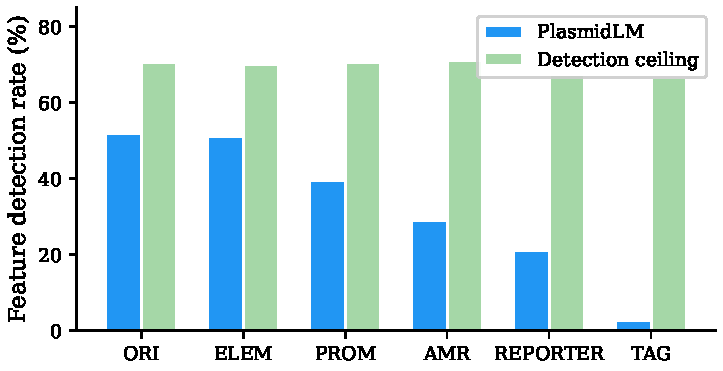
\includegraphics[width=0.85\linewidth]{figures/prompt_fidelity_ceiling.pdf}
  \caption{``Faithful plasmid'' rate vs.\ fidelity threshold $T$ for both checkpoints
    with paired bootstrap $95\%$ bands (left), and the paired GRPO$-$base delta across $T$
  (right). The effect peaks near $T=0.5$ and is significant at every positive threshold.}
  \label{fig:ceiling}
\end{figure}

\begin{figure}[ht]
  \centering
  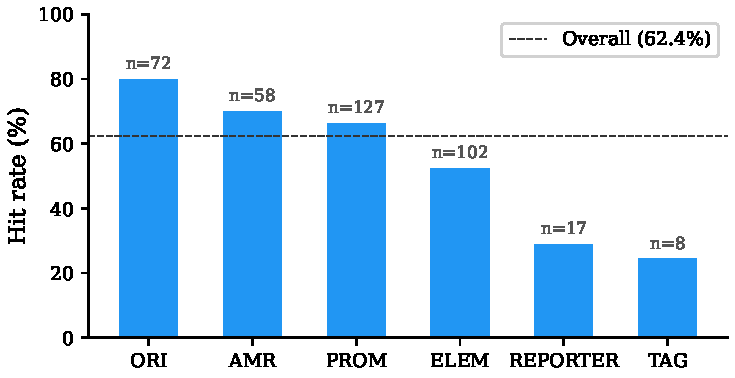
\includegraphics[width=0.85\linewidth]{figures/hit_rate_by_category.pdf}
  \caption{Per-category prompt faithfulness on the held-out $1{,}000$-prompt benchmark,
    supervised base versus post-GRPO. Error bars are Wilson $95\%$ intervals on pooled
    counts; see Appendix~\ref{app:stats} for the non-independence caveat.}
  \label{fig:hit_rate}
\end{figure}

\begin{figure}[ht]
  \centering
  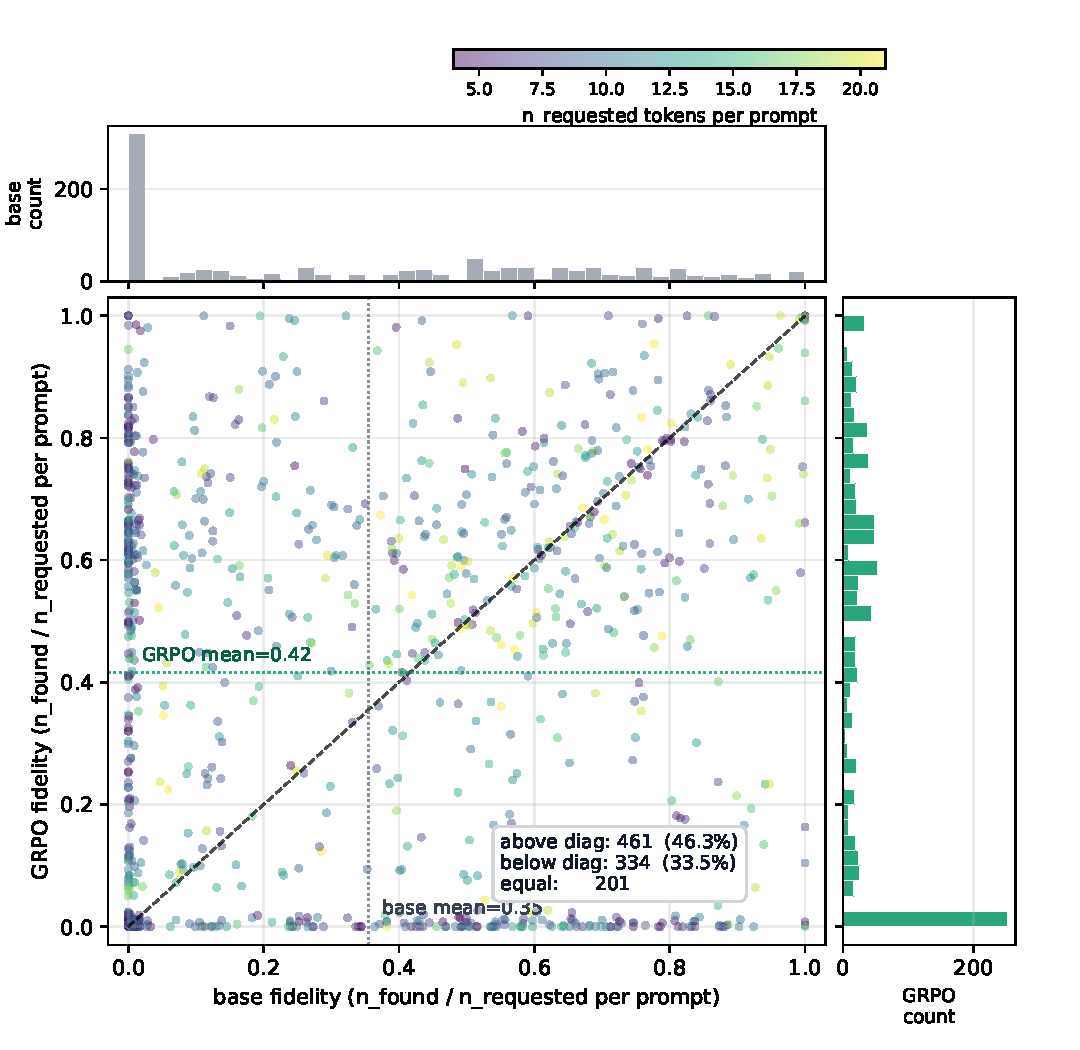
\includegraphics[width=0.80\linewidth]{figures/fidelity_scatter.pdf}
  \caption{Per-prompt faithfulness on the held-out $1{,}000$-prompt benchmark,
    supervised base ($x$-axis) vs.\ post-GRPO ($y$-axis). Marker jitter separates points
    landing on shared fractions (e.g.\ $1/2$, $2/3$). Point colour encodes the number of
    tokens requested per prompt; marginal histograms show each model's univariate
    distribution. $46.3\%$ of prompts improve under post-training, $33.5\%$ regress, and
    $20.1\%$ are unchanged; the improvement is broadly distributed across prompt
    complexity rather than concentrated on simple prompts.}
  \label{fig:scatter}
\end{figure}

\subsection{Base-model temperature sweep}
\label{app:tempsweep}

\begin{figure}[ht]
  \centering
  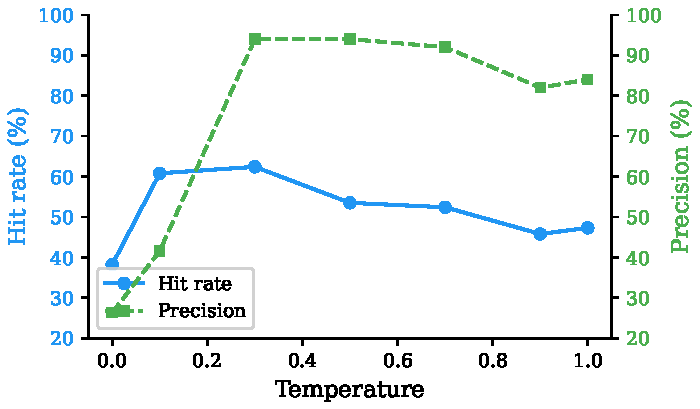
\includegraphics[width=0.85\linewidth]{figures/temperature_sweep.pdf}
  \caption{Pre-GRPO base model, small temperature sweep ($n=100$ per cell; matched
    $n=1000$ run for $t=0.7$ for comparison). Base prompt fidelity peaks at $t=0.3$
    ($37.8\%$) and degrades at higher temperatures; the matched $t=0.7$ setting is
    therefore already near the base's optimum, so the GRPO advantage reported in the main
  text is not explained by temperature tuning on the base.}
  \label{fig:temperature_sweep}
\end{figure}

\section{Statistical conventions}
\label{app:stats}

Wilson $95\%$ CIs on rates; paired bootstrap CIs ($10{,}000$ resamples, resampling
prompts) on binary-outcome deltas; McNemar with continuity correction (exact when any
cell $<25$) on paired binary contingency tables. Per-sequence faithfulness CIs are
bootstrapped over prompts because tokens within a prompt are not independent. The
per-category hit-rate table reports raw token-pooled rates without CIs for the same
reason; per-category Wilson intervals on pooled counts (used in
Figure~\ref{fig:hit_rate}) are mildly optimistic and flagged as such. All artefacts are
archived and will be released upon acceptance.

\section{Per-token hit-rate decomposition}
\label{app:pertoken}

\begin{figure}[ht]
  \centering
  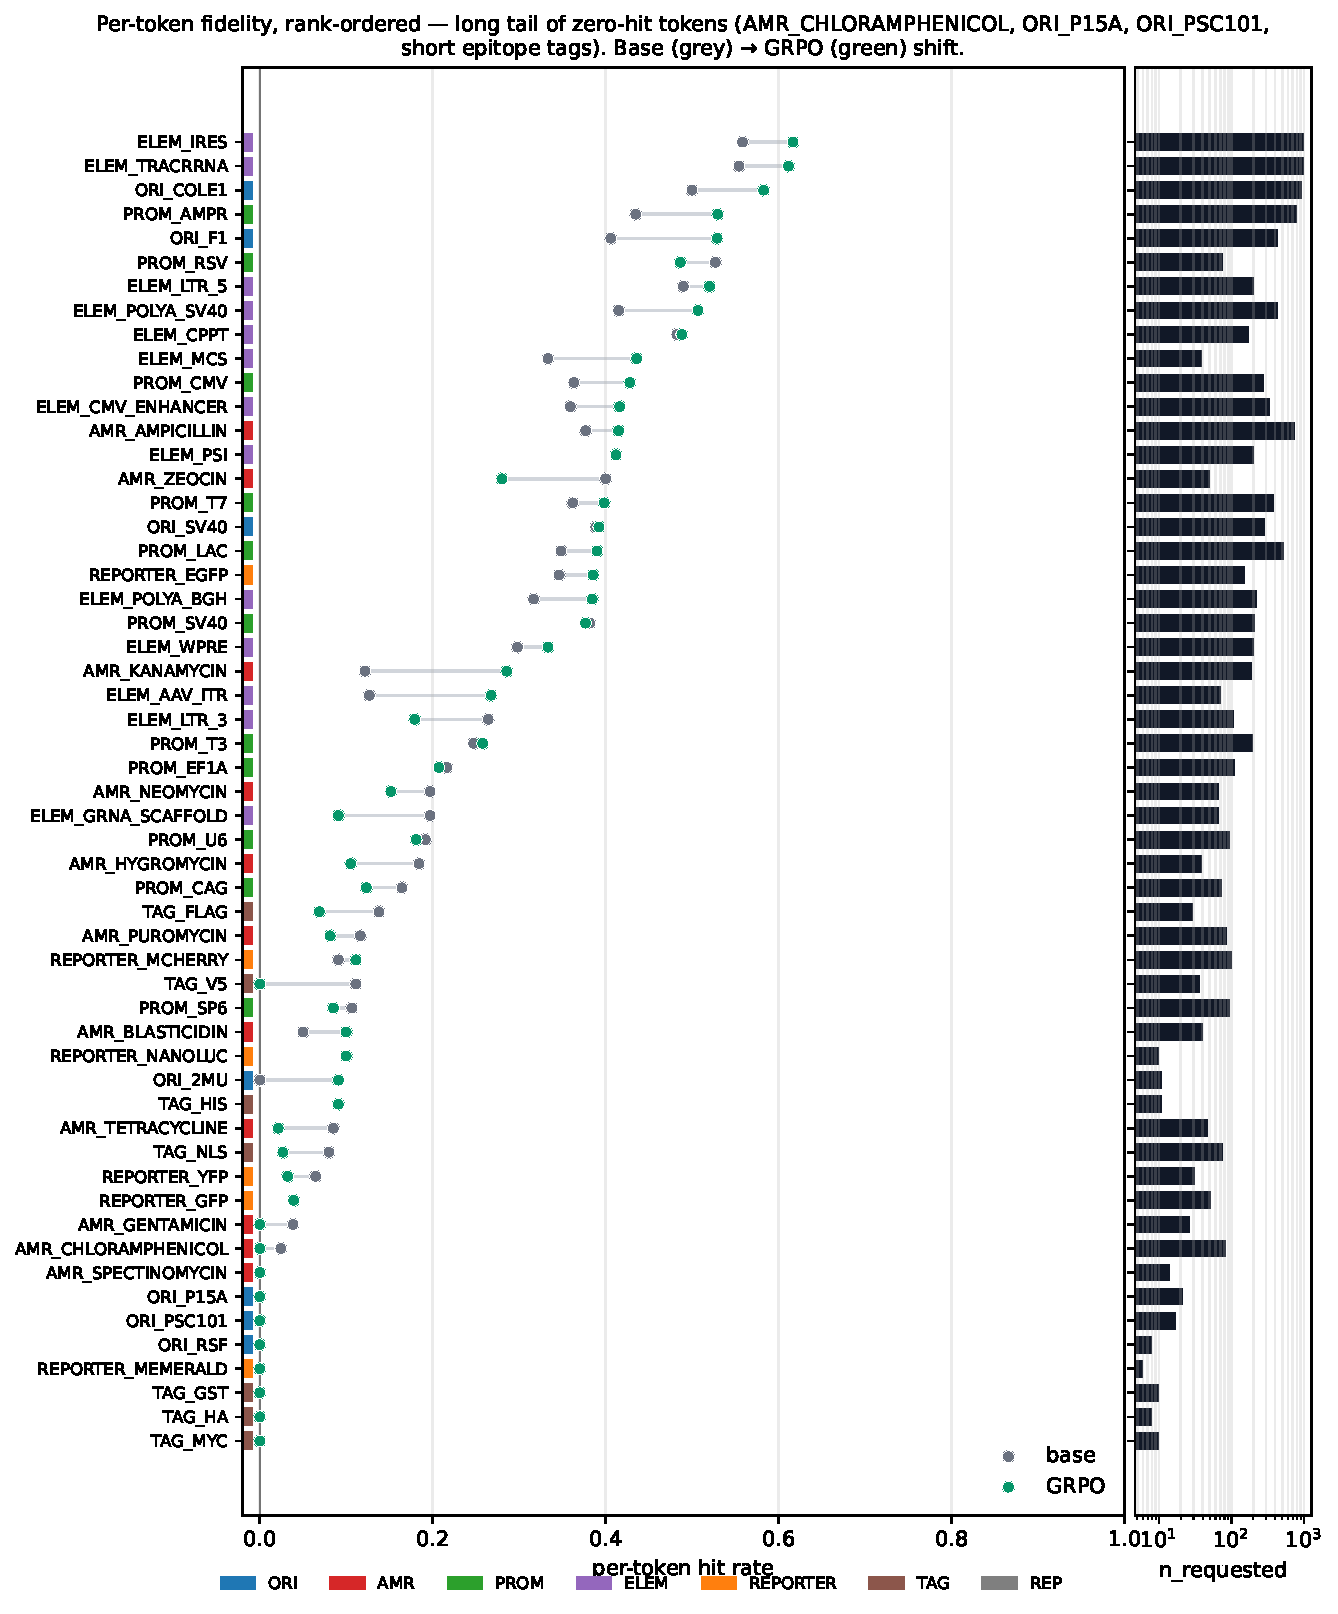
\includegraphics[width=0.88\linewidth]{figures/per_token_hit_rates.pdf}
  \caption{Per-token hit rate, rank-ordered by the maximum of the base and GRPO rates.
    Each row shows one hard token: base (grey) and GRPO (green) dots connected by a light
    line to highlight the shift. Category colour strip on the far left. Right panel is
    $n_{\text{requested}}$ in the paired eval on a log scale. The figure makes two patterns
    visible: GRPO uniformly lifts the already-detectable tokens, and a long tail of rare
    tokens stays at zero in both runs (the zero-hit tail is the same set that explains the
  TAG regression and the \texttt{COPY\_LOW} soft-token failure in Section~\ref{sec:soft-tokens}).}
  \label{fig:per-token}
\end{figure}

\begin{figure}[ht]
  \centering
  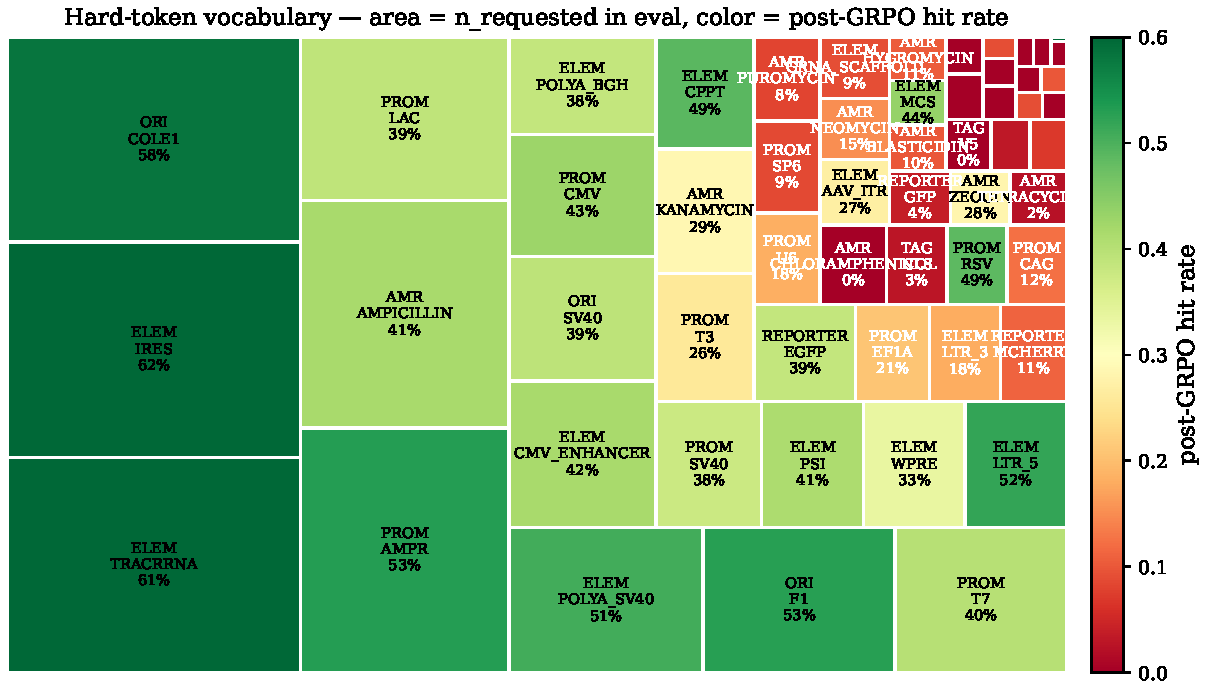
\includegraphics[width=\linewidth]{figures/vocab_treemap.pdf}
  \caption{Hard-token vocabulary scope on the held-out benchmark, as a treemap. Tile
    area is the number of times the token appears in evaluation prompts; tile colour
    is the post-GRPO hit rate ($0$--$60\%$ red$\to$green scale). The four large green
    tiles in the upper-left (\texttt{ELEM\_TRACRRNA}, \texttt{ELEM\_IRES},
    \texttt{ORI\_COLE1}, \texttt{PROM\_AMPR}) carry most of the evaluation mass and
    achieve $50$--$58\%$ hit rates. The long tail of small dark tiles on the right is
    the zero-hit set: rare antibiotic resistance markers, rare origins, and most short
    epitope tags. \texttt{REP\_*} tokens have no evaluation prompts and are omitted.
    Companion to Figure~\ref{fig:per-token}, which shows base$\to$GRPO movement; the
    treemap shows scope of vocabulary at a glance.}
  \label{fig:vocab_treemap}
\end{figure}

\section{Soft-token conditioning analysis}
\label{app:softtokens}

\paragraph{Probe construction.} For each soft value (e.g., \texttt{VEC\_LENTIVIRAL}) we
list the hard-token signature biology expects: LTRs, $\Psi$, cPPT, and WPRE in this case.
Each hard token resolves to a set of pLannotate sseqids via the motif registry; the
soft-value probe is the union of those sseqid sets. We then compare the probe-hit rate
between prompts carrying the soft value and prompts carrying a different value in the
same soft category, using Fisher's exact (two-sided). Probes for tags without
biologically exclusive signatures (e.g.\ \texttt{VEC\_MAMMALIAN}, whose features appear
in most plasmids for unrelated reasons) are included for completeness but are expected to
wash out. Four soft categories are defined in the vocabulary: \texttt{BB\_*} ($20$
values), \texttt{COPY\_\{HIGH,LOW\}}, \texttt{SP\_*} ($9$ values), \texttt{VEC\_*} ($11$ values).

\begin{figure}[ht]
  \centering
  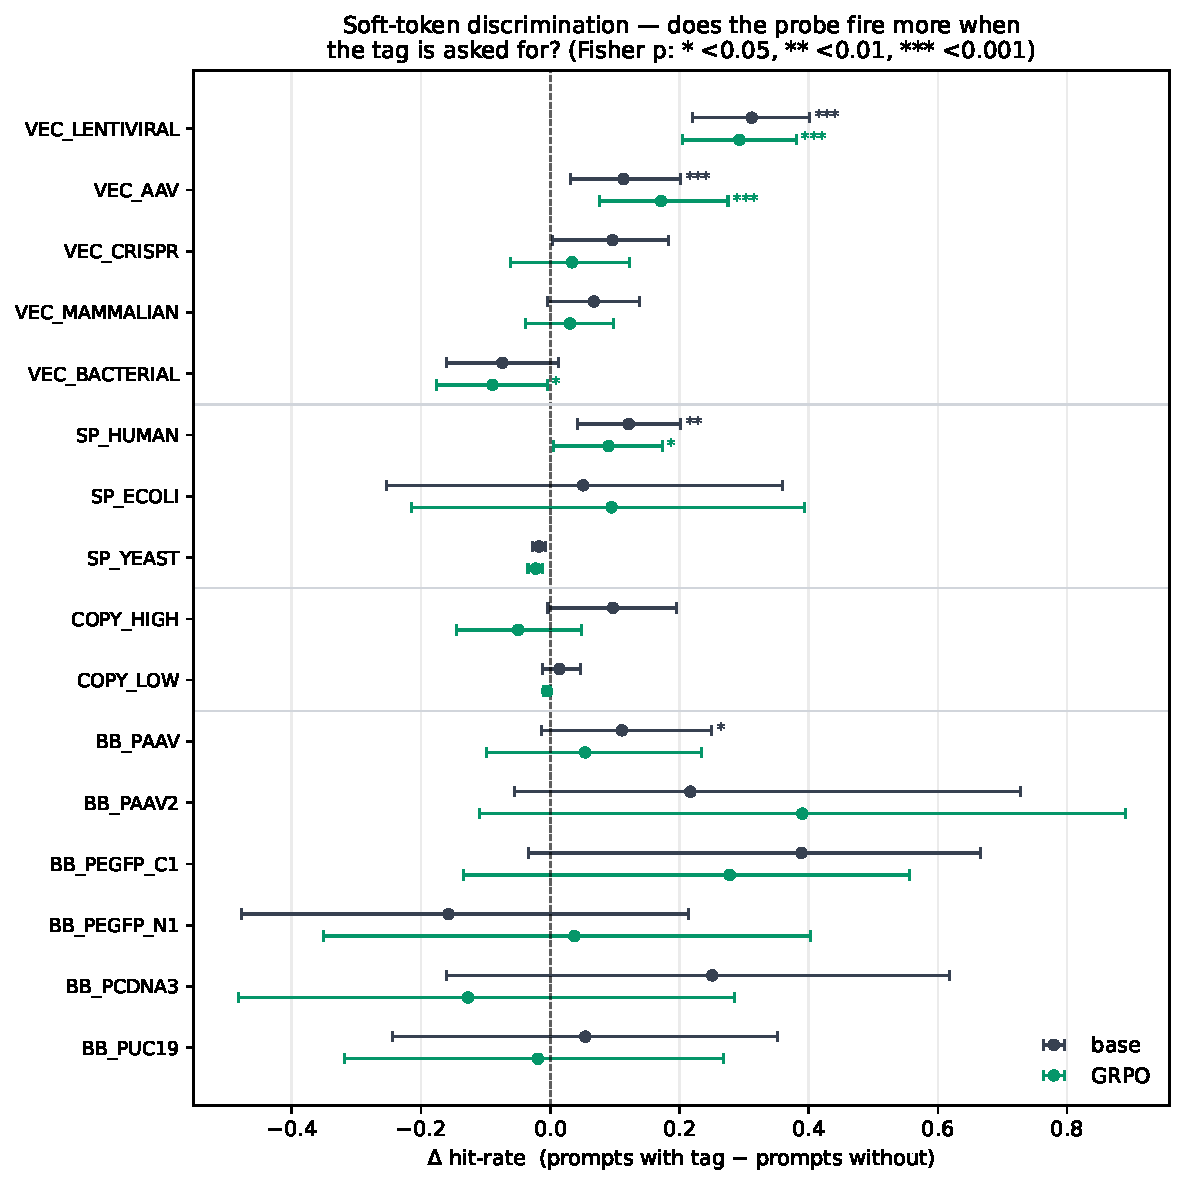
\includegraphics[width=0.88\linewidth]{figures/soft_token_forest.pdf}
  \caption{Soft-token discrimination. For each soft value with a biologically meaningful
    probe, $\Delta$ is the difference in probe-hit rate between prompts that carry that tag
    and prompts that carry some other value in the same category; error bars are bootstrap
    $95\%$ intervals; stars mark Fisher $p<0.05$ ($\ast$), $<0.01$ ($\ast\ast$), $<0.001$
    ($\ast\ast\ast$). \texttt{VEC\_LENTIVIRAL} and \texttt{VEC\_AAV} show large,
    significant conditioning effects in both the pretrained base and the post-GRPO model.
    Most other tags are indistinguishable from zero; GRPO preserves but does not extend the
  pattern, consistent with soft tokens being absent from the reward.}
  \label{fig:soft-token-forest}
\end{figure}

\begin{figure}[ht]
  \centering
  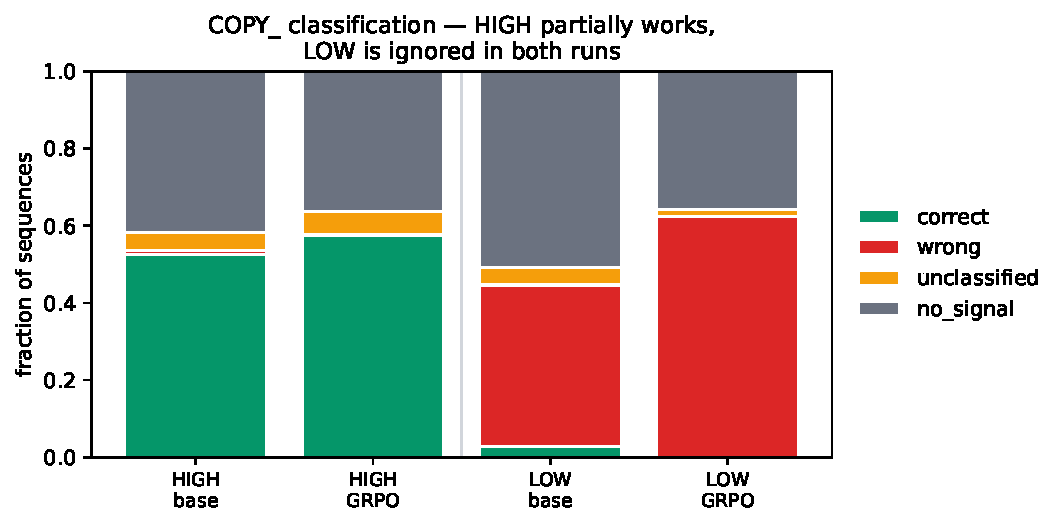
\includegraphics[width=0.72\linewidth]{figures/soft_token_copy_buckets.pdf}
  \caption{\texttt{COPY\_} conditioning, stacked by outcome. \emph{correct} = the
    requested copy class's origin was detected; \emph{wrong} = the opposing class's origin
    was detected instead; \emph{unclassified} = a non-discriminative origin (e.g.\ ORI\_F1,
    ORI\_SV40, ORI\_2$\mu$) was detected; \emph{no\_signal} = no origin detected.
    \texttt{COPY\_HIGH} partially works in both runs; \texttt{COPY\_LOW} is effectively
    ignored, with the model outputting a high-copy origin far more often than a low-copy
  one when low copy is requested.}
  \label{fig:soft-token-copy}
\end{figure}

\section{Evaluation pipeline and reproducibility}
\label{app:pipeline}

The complete evaluation pipeline constructs reference panels and negative controls,
performs large-scale generation and annotation with pLannotate, Prodigal, and dustmasker,
computes viability and fidelity metrics, trains the LightGBM discriminator, and computes
best-of-$K$ tables. All artifacts (generations, pLannotate JSON, per-prompt fidelity
parquets, discriminator outputs) are archived in an anonymized repository and will be
released upon acceptance. Commands, random seeds, and environment specifications are
included. The best-of-$K$ analysis is runnable end-to-end as a PEP 723 script at
\texttt{eval/scripts/analyze\_best\_of\_k.py}; the paired marimo notebook
\texttt{notebooks/base\_vs\_grpo\_analysis.py} renders every figure and table in
Section~\ref{sec:useful} directly from the archived data.

\paragraph{Folding protocol.} MFE density is computed with ViennaRNA's
\texttt{fold} under the DNA Mathews 2004 parameter set; sequences $\le 5$ kb are
folded full-length, longer sequences are summarised as the mean MFE density across $5$
random $2$ kb windows.

\paragraph{GRPO training run note.} The released checkpoint was produced by a run whose
experiment tracking logs were not retained. The training configuration in
Table~\ref{tab:hyperparams} was reconstructed from the git commit whose on-disk config
file byte-matches the uploaded \texttt{model.safetensors}; this configuration is
committed to the HuggingFace model repository as \texttt{training\_config.py} for
reference. The training procedure is fully reproducible from this config.

%%%%%%%%%%%%%%%%%%%%%%%%%%%%%%%%%%%%%%%%%%%%%%%%%%%%%%%%%%%%

\newpage
\section*{NeurIPS Paper Checklist}

%%% BEGIN INSTRUCTIONS %%%
The checklist is designed to encourage best practices for responsible machine learning research, addressing issues of reproducibility, transparency, research ethics, and societal impact. Do not remove the checklist: {\bf The papers not including the checklist will be desk rejected.} The checklist should follow the references and follow the (optional) supplemental material.  The checklist does NOT count towards the page
limit. 

Please read the checklist guidelines carefully for information on how to answer these questions. For each question in the checklist:
\begin{itemize}
    \item You should answer \answerYes{}, \answerNo{}, or \answerNA{}.
    \item \answerNA{} means either that the question is Not Applicable for that particular paper or the relevant information is Not Available.
    \item Please provide a short (1--2 sentence) justification right after your answer (even for \answerNA). 
   % \item {\bf The papers not including the checklist will be desk rejected.}
\end{itemize}

{\bf The checklist answers are an integral part of your paper submission.} They are visible to the reviewers, area chairs, senior area chairs, and ethics reviewers. You will also be asked to include it (after eventual revisions) with the final version of your paper, and its final version will be published with the paper.

The reviewers of your paper will be asked to use the checklist as one of the factors in their evaluation. While \answerYes{} is generally preferable to \answerNo{}, it is perfectly acceptable to answer \answerNo{} provided a proper justification is given (e.g., error bars are not reported because it would be too computationally expensive'' or ``we were unable to find the license for the dataset we used''). In general, answering \answerNo{} or \answerNA{} is not grounds for rejection. While the questions are phrased in a binary way, we acknowledge that the true answer is often more nuanced, so please just use your best judgment and write a justification to elaborate. All supporting evidence can appear either in the main paper or the supplemental material, provided in appendix. If you answer \answerYes{} to a question, in the justification please point to the section(s) where related material for the question can be found.

IMPORTANT, please:
\begin{itemize}
    \item {\bf Delete this instruction block, but keep the section heading ``NeurIPS Paper Checklist"},
    \item  {\bf Keep the checklist subsection headings, questions/answers and guidelines below.}
    \item {\bf Do not modify the questions and only use the provided macros for your answers}.
\end{itemize} 
 

%%% END INSTRUCTIONS %%%


\begin{enumerate}

\item {\bf Claims}
    \item[] Question: Do the main claims made in the abstract and introduction accurately reflect the paper's contributions and scope?
    \item[] Answer: \answerYes{}
    \item[] Justification: The abstract and introduction clearly articulate the testbed role of plasmids for controllable DNA generation, the shift from predictive to instruction-following models via GRPO with automated rewards, the dual viability and prompt-fidelity evaluation axes, and key quantitative results (plausibility $56.8\% \to 59.6\%$, prompt fidelity $35.5\% \to 41.6\%$, composite useful-plasmid rate $38.7\% \to 48.5\%$, and best-of-$K{=}4$ $78.9\% \to 89.7\%$). Limitations (detection ceilings, lack of wet-lab validation, data bias, non-uniform soft-token controllability) are explicitly discussed in the Introduction, Experiments, and Discussion sections. Claims are supported by experiments in Sections~\ref{sec:eval}--\ref{sec:experiments} and archived evaluation results.
    \item[] Guidelines: See above.

\item {\bf Limitations}
    \item[] Question: Does the paper discuss the limitations of the work performed by the authors?
    \item[] Answer: \answerYes{}
    \item[] Justification: A dedicated Discussion section (Section~\ref{sec:discussion}) and parts of the Introduction and Experiments explicitly address limitations including computational-only evaluation (no wet-lab validation), detection ceilings of automated annotators ($\sim$72\% on real data), training data bias toward common lab plasmids, linear vs circular representation, context length limits, and the inherent interplay/trade-offs between viability and prompt fidelity. The appendix provides further pipeline details. See also the NeurIPS checklist entry on broader impact.
    \item[] Guidelines:
    \begin{itemize}
        \item The answer \answerNA{} means that the paper has no limitation while the answer \answerNo{} means that the paper has limitations, but those are not discussed in the paper. 
        \item The authors are encouraged to create a separate ``Limitations'' section in their paper.
        \item The paper should point out any strong assumptions and how robust the results are to violations of these assumptions (e.g., independence assumptions, noiseless settings, model well-specification, asymptotic approximations only holding locally). The authors should reflect on how these assumptions might be violated in practice and what the implications would be.
        \item The authors should reflect on the scope of the claims made, e.g., if the approach was only tested on a few datasets or with a few runs. In general, empirical results often depend on implicit assumptions, which should be articulated.
        \item The authors should reflect on the factors that influence the performance of the approach. For example, a facial recognition algorithm may perform poorly when image resolution is low or images are taken in low lighting. Or a speech-to-text system might not be used reliably to provide closed captions for online lectures because it fails to handle technical jargon.
        \item The authors should discuss the computational efficiency of the proposed algorithms and how they scale with dataset size.
        \item If applicable, the authors should discuss possible limitations of their approach to address problems of privacy and fairness.
        \item While the authors might fear that complete honesty about limitations might be used by reviewers as grounds for rejection, a worse outcome might be that reviewers discover limitations that aren't acknowledged in the paper. The authors should use their best judgment and recognize that individual actions in favor of transparency play an important role in developing norms that preserve the integrity of the community. Reviewers will be specifically instructed to not penalize honesty concerning limitations.
    \end{itemize}

\item {\bf Theory assumptions and proofs}
    \item[] Question: For each theoretical result, does the paper provide the full set of assumptions and a complete (and correct) proof?
    \item[] Answer: \answerNA{}
    \item[] Justification: No theoretical results or proofs in the paper.
    \item[] Guidelines:
    \begin{itemize}
        \item The answer \answerNA{} means that the paper does not include theoretical results. 
        \item All the theorems, formulas, and proofs in the paper should be numbered and cross-referenced.
        \item All assumptions should be clearly stated or referenced in the statement of any theorems.
        \item The proofs can either appear in the main paper or the supplemental material, but if they appear in the supplemental material, the authors are encouraged to provide a short proof sketch to provide intuition. 
        \item Inversely, any informal proof provided in the core of the paper should be complemented by formal proofs provided in appendix or supplemental material.
        \item Theorems and Lemmas that the proof relies upon should be properly referenced. 
    \end{itemize}

    \item {\bf Experimental result reproducibility}
    \item[] Question: Does the paper fully disclose all the information needed to reproduce the main experimental results of the paper to the extent that it affects the main claims and/or conclusions of the paper (regardless of whether the code and data are provided or not)?
    \item[] Answer: \answerYes{}
    \item[] Justification: All necessary details are provided in Section~\ref{sec:methods}, Section~\ref{sec:eval}, and the appendix: dataset, tokenizer, architecture, training hyperparameters, GRPO scorer definitions, inference settings (temperature, top-$p$, top-$k$), alignment thresholds, baseline construction, and evaluation metrics. Code and data are released publicly.
    \item[] Guidelines:
    \begin{itemize}
        \item The answer \answerNA{} means that the paper does not include experiments.
        \item If the paper includes experiments, a \answerNo{} answer to this question will not be perceived well by the reviewers: Making the paper reproducible is important, regardless of whether the code and data are provided or not.
        \item If the contribution is a dataset and\slash or model, the authors should describe the steps taken to make their results reproducible or verifiable. 
        \item Depending on the contribution, reproducibility can be accomplished in various ways. For example, if the contribution is a novel architecture, describing the architecture fully might suffice, or if the contribution is a specific model and empirical evaluation, it may be necessary to either make it possible for others to replicate the model with the same dataset, or provide access to the model. In general. releasing code and data is often one good way to accomplish this, but reproducibility can also be provided via detailed instructions for how to replicate the results, access to a hosted model (e.g., in the case of a large language model), releasing of a model checkpoint, or other means that are appropriate to the research performed.
        \item While NeurIPS does not require releasing code, the conference does require all submissions to provide some reasonable avenue for reproducibility, which may depend on the nature of the contribution. For example
        \begin{enumerate}
            \item If the contribution is primarily a new algorithm, the paper should make it clear how to reproduce that algorithm.
            \item If the contribution is primarily a new model architecture, the paper should describe the architecture clearly and fully.
            \item If the contribution is a new model (e.g., a large language model), then there should either be a way to access this model for reproducing the results or a way to reproduce the model (e.g., with an open-source dataset or instructions for how to construct the dataset).
            \item We recognize that reproducibility may be tricky in some cases, in which case authors are welcome to describe the particular way they provide for reproducibility. In the case of closed-source models, it may be that access to the model is limited in some way (e.g., to registered users), but it should be possible for other researchers to have some path to reproducing or verifying the results.
        \end{enumerate}
    \end{itemize}


\item {\bf Open access to data and code}
    \item[] Question: Does the paper provide open access to the data and code, with sufficient instructions to faithfully reproduce the main experimental results, as described in supplemental material?
    \item[] Answer: \answerYes{}
    \item[] Justification: The model, tokenizer, GRPO training code, scorers, evaluation pipeline, and archived evaluation data are released publicly with reproducibility instructions. Dataset (Addgene plasmids) is publicly available. The appendix details the pipeline and points to the Hugging Face bucket.
    \item[] Guidelines:
    \begin{itemize}
        \item The answer \answerNA{} means that paper does not include experiments requiring code.
        \item Please see the NeurIPS code and data submission guidelines (\url{https://neurips.cc/public/guides/CodeSubmissionPolicy}) for more details.
        \item While we encourage the release of code and data, we understand that this might not be possible, so \answerNo{} is an acceptable answer. Papers cannot be rejected simply for not including code, unless this is central to the contribution (e.g., for a new open-source benchmark).
        \item The instructions should contain the exact command and environment needed to run to reproduce the results. See the NeurIPS code and data submission guidelines (\url{https://neurips.cc/public/guides/CodeSubmissionPolicy}) for more details.
        \item The authors should provide instructions on data access and preparation, including how to access the raw data, preprocessed data, intermediate data, and generated data, etc.
        \item The authors should provide scripts to reproduce all experimental results for the new proposed method and baselines. If only a subset of experiments are reproducible, they should state which ones are omitted from the script and why.
        \item At submission time, to preserve anonymity, the authors should release anonymized versions (if applicable).
        \item Providing as much information as possible in supplemental material (appended to the paper) is recommended, but including URLs to data and code is permitted.
    \end{itemize}


\item {\bf Experimental setting/details}
    \item[] Question: Does the paper specify all the training and test details (e.g., data splits, hyperparameters, how they were chosen, type of optimizer) necessary to understand the results?
    \item[] Answer: \answerYes{}
    \item[] Justification: Methods (Section~\ref{sec:methods}), Experimental Setup (Section~\ref{sec:eval}), and Appendix (Table~\ref{tab:hyperparams}) provide full details on the dataset (108,448 Addgene plasmids), tokenizer, 19.3M model architecture, pretraining (65{,}000 steps, AdamW, cosine LR, peak $3\times10^{-4}$), GRPO ($G{=}8$, KL $\beta{=}0.5$, pLannotate composite reward against the motif registry), inference, baselines, temperatures, alignment thresholds, and evaluation pipeline.
    \item[] Guidelines: See above.

\item {\bf Experiment statistical significance}
    \item[] Question: Does the paper report error bars suitably and correctly defined or other appropriate information about the statistical significance of the experiments?
    \item[] Answer: \answerYes{}
    \item[] Justification: The paired $n{=}1{,}000$ evaluation reports Wilson $95\%$ confidence intervals on all rates, paired bootstrap $95\%$ CIs on deltas, and McNemar $p$-values on all binary paired comparisons (plausibility, fidelity at every threshold, best-of-$K$ at $K\in\{1,2,4\}$). Four independent seeds per model are used for the best-of-$K$ analysis and to confirm plausibility run-to-run standard deviation ($\approx 1$ pp). The per-sequence fidelity CI is bootstrapped over the $996$ prompts that contain at least one hard token; the per-category hit-rate CIs are Wilson intervals on token-pooled counts, with the non-independence of tokens within a prompt explicitly flagged in Section~\ref{sec:eval}.
    \item[] Guidelines: See above.

\item {\bf Experiments compute resources}
    \item[] Question: For each experiment, does the paper provide sufficient information on the computer resources (type of compute workers, memory, time of execution) needed to reproduce the experiments?
    \item[] Answer: \answerYes{}
    \item[] Justification: Methods and Appendix specify compute: pretraining $\sim$35 hours on $1{\times}$A100-40GB ($65{,}000$ steps), GRPO post-training $\sim$17 hours on a single GPU (Anyscale), generation $\sim$46 min for $1{,}000$ sequences, and the full evaluation pipeline (pLannotate + Prodigal + dustmasker + downstream metrics) on the $1{,}000$-sequence eval in approximately two hours on a single machine. Full configs and scripts are in the repository.
    \item[] Guidelines: See above.
    
\item {\bf Code of ethics}
    \item[] Question: Does the research conducted in the paper conform, in every respect, with the NeurIPS Code of Ethics \url{https://neurips.cc/public/EthicsGuidelines}?
    \item[] Answer: \answerYes{}
    \item[] Justification: Work uses public Addgene data and open tools. Broader impacts and dual-use considerations (synthetic biology) are discussed in Section~\ref{sec:discussion}. No human subjects research. Model release includes comprehensive evaluation to promote responsible use. Anonymity preserved for review.
    \item[] Guidelines: See above.


\item {\bf Broader impacts}
    \item[] Question: Does the paper discuss both potential positive societal impacts and negative societal impacts of the work performed?
    \item[] Answer: \answerYes{}
    \item[] Justification: Section~\ref{sec:discussion} discusses positive impacts (advancing designable DNA, reducing reliance on manual/template cloning in synthetic biology) and negative ones (potential dual-use for harmful constructs, training data bias toward common lab plasmids). Mitigation strategies including open release with evaluation suite, wet-lab validation emphasis, and curriculum learning are addressed.
    \item[] Guidelines: See above.
    
\item {\bf Safeguards}
    \item[] Question: Does the paper describe safeguards that have been put in place for responsible release of data or models that have a high risk for misuse (e.g., pre-trained language models, image generators, or scraped datasets)?
    \item[] Answer: \answerYes{}
    \item[] Justification: The 19M-parameter model is released alongside the full open-source evaluation suite, scorers (including the binary motif scorer and alignment scorer), and detailed limitations in Section~\ref{sec:discussion} and the appendix. No scraped data is used.
    \item[] Guidelines: See above.

\item {\bf Licenses for existing assets}
    \item[] Question: Are the creators or original owners of assets (e.g., code, data, models), used in the paper, properly credited and are the license and terms of use explicitly mentioned and properly respected?
    \item[] Answer: \answerYes{}
    \item[] Justification: Addgene is cited; pLannotate, parasail, ViennaRNA, sourmash, LightGBM, and all other tools are properly referenced with original papers. Repository includes licenses for all released code, model, and evaluation data.
    \item[] Guidelines: See above.

\item {\bf New assets}
    \item[] Question: Are new assets introduced in the paper well documented and is the documentation provided alongside the assets?
    \item[] Answer: \answerYes{}
    \item[] Justification: The PlasmidLM model, custom tokenizer, GRPO infrastructure, scorers (including alignment and binary motif variants), evaluation pipeline, and archived data are released with full documentation, training details, limitations, and reproducibility instructions in the repository, paper, and appendix.
    \item[] Guidelines: See above.

\item {\bf Crowdsourcing and research with human subjects}
    \item[] Question: For crowdsourcing experiments and research with human subjects, does the paper include the full text of instructions given to participants and screenshots, if applicable, as well as details about compensation (if any)? 
    \item[] Answer: \answerNA{}
    \item[] Justification: No crowdsourcing or human subjects research.
    \item[] Guidelines: See above.

\item {\bf Institutional review board (IRB) approvals or equivalent for research with human subjects}
    \item[] Question: Does the paper describe potential risks incurred by study participants, whether such risks were disclosed to the subjects, and whether Institutional Review Board (IRB) approvals (or an equivalent approval/review based on the requirements of your country or institution) were obtained?
    \item[] Answer: \answerNA{}
    \item[] Justification: No human subjects research.
    \item[] Guidelines: See above.

\item {\bf Declaration of LLM usage}
    \item[] Question: Does the paper describe the usage of LLMs if it is an important, original, or non-standard component of the core methods in this research? Note that if the LLM is used only for writing, editing, or formatting purposes and does \emph{not} impact the core methodology, scientific rigor, or originality of the research, declaration is not required.
    %this research? 
    \item[] Answer: \answerNA{}
    \item[] Justification: No theoretical results or proofs in the paper.
    \item[] Guidelines:
    \begin{itemize}
        \item The answer \answerNA{} means that the core method development in this research does not involve LLMs as any important, original, or non-standard components.
        \item Please refer to our LLM policy in the NeurIPS handbook for what should or should not be described.
    \end{itemize}

\end{enumerate}

\end{document}
